\RequirePackage{amsthm} %https://tex.stackexchange.com/questions/687324/unknown-theoremstyle-warning-with-springer-nature-template
\documentclass[sn-mathphys-num,iicol]{sn-jnl}

%\usepackage{sn-jnl.sty}
\usepackage{graphicx}%
\usepackage{multirow}%
\usepackage{amsmath,amssymb,amsfonts}%
\usepackage{amsthm}%
\usepackage{physics}
\usepackage{siunitx}
\usepackage{mathrsfs}%
\usepackage[title]{appendix}%
\usepackage{xcolor}%
\usepackage{textcomp}%
\usepackage{manyfoot}%
\usepackage{booktabs}%
\usepackage{algorithm}%
\usepackage{algorithmicx}%
\usepackage{algpseudocode}%
\usepackage{listings}%
\usepackage{newtxmath}%
\usepackage[tiny]{titlesec}%
\usepackage[ngerman]{babel}

\theoremstyle{thmstyleone}
\newtheorem{theorem}{Theorem}
\newtheorem{proposition}[theorem]{Proposition}

\theoremstyle{thmstyletwo}
\newtheorem{remark}{Remark}

\theoremstyle{thmstylethree}
\newtheorem{definition}{Definition}

\raggedbottom

\newcommand{\td}{\text{d}}

\titleformat{\subsection}{}{\thesubsection}{1em}{\itshape}
\titleformat{\subsubsection}{}{\thesubsubsection}{1em}{\itshape}

\begin{document}
        
\title{Praktikum 4 -- Versuch 402: Quantelung von Energie}
\author*[1]{\fnm{Jonas} \sur{Wortmann}}\email{s02jwort@uni-bonn.de}
\author*[1]{\fnm{Angelo} \sur{Brade}}\email{s72abrad@uni-bonn.de}
\affil*[1]{Rheinische Friedrich--Wilhelms--Universität, Bonn}
\maketitle

\newpage
\section{Einleitung}
Elektronen emittieren bzw.\ absorbieren beim Übergang zwischen Orbitalen Photonen mit einer diskreten Energie.
Diese Energie ist gequantelt in Vielfache des \textsc{Planck}'schen Wirkungsquantums $h$.
Um die Größe der Quantelung zu bestimmen wird der Photoeffekt und die Messung der \textsc{Balmer}--Serie von Hg verwendet.

\section{Photoelektrische Bestimmung von $h$.} \label{sec:photoeffekt}
\subsection{Theoretischer Hintergrund}
Das \textsc{Fermi}--Niveau beschreibt das höchste Energieniveau in einem Atom im Grundzustand, welches aufgrund des \textsc{Pauli}--Prinzips noch besetzt werden darf.
Die Austrittsarbeit ist die Arbeit die benötigt wird, um ein Elektron aus diesem Energieniveau zu heben und vom dem Atoms zu lösen.
Für verschiedene Atome ist dieses Level, wegen ihrer unterschiedlichen Elektronanzahl, nicht gleich.
Makroskopisch zeigt sich dies in unterschiedlichen Austrittsarbeiten für verschiedene Materialien, wie z.B.\ für die Anode und die Kathode im experimentellen Aufbau.

Solche Energieniveaus können mit dem Bänderschema verdeutlicht werden.
Eine mögliche Anordnung ist in Abb.\ (\ref{fig:bänderschema}) gezeigt.
Die gestrichelten Linien unten mit den schrägen Linien darunter geben die jeweiligen \textsc{Fermi}--Niveaus an.
$W_\text{K}$ und $W_\text{A}$ geben die Austrittsarbeit an.
Die alleinstehende gestrichelte Linie ist das Vakuumniveau.

Werden Anode und Kathode miteinander verbunden, so gleichen sich ihre \textsc{Fermi}--Niveaus aus und es entsteht eine Potentialdifferenz von $U_\text{KA}$ zum Vakuumsniveau zwischen Anode und Kathode.
Wird eine Spannung zwischen Anode und Kathode aufgebaut, so verschieben sich die \textsc{Fermi}--Niveaus und es baut sich eine weitere Potentialdifferenz $U_\text{G}$ auf.

Der Photoeffekt beschreibt folgendes Phänomen: Trifft ein Photon auf die Kathode, so lässt sich eine Gleichung zwischen der Energie des Photons und der Energie des Elektrons aufstellen, mit $eU_0$ der kinetischen Energie der Elektronen
\begin{align} 
        \Leftrightarrow && E_\gamma =h\nu &=eU_0-eU_\text{KA}+W_\text{K}=E_{e^-}&&\\
        \Leftrightarrow &&&=eU_0-\left(W_\text{K}-W_\text{A}\right)+W_\text{K}&&\\
        \Leftrightarrow &&&=eU_0+W_\text{A}.&&
\end{align} 
Dem Photon ist es also bei einer ausgezeichneten Energie möglich das Elektron aus dem \textsc{Fermi}--Niveau zu heben.
\begin{figure}[t]
        \centering
        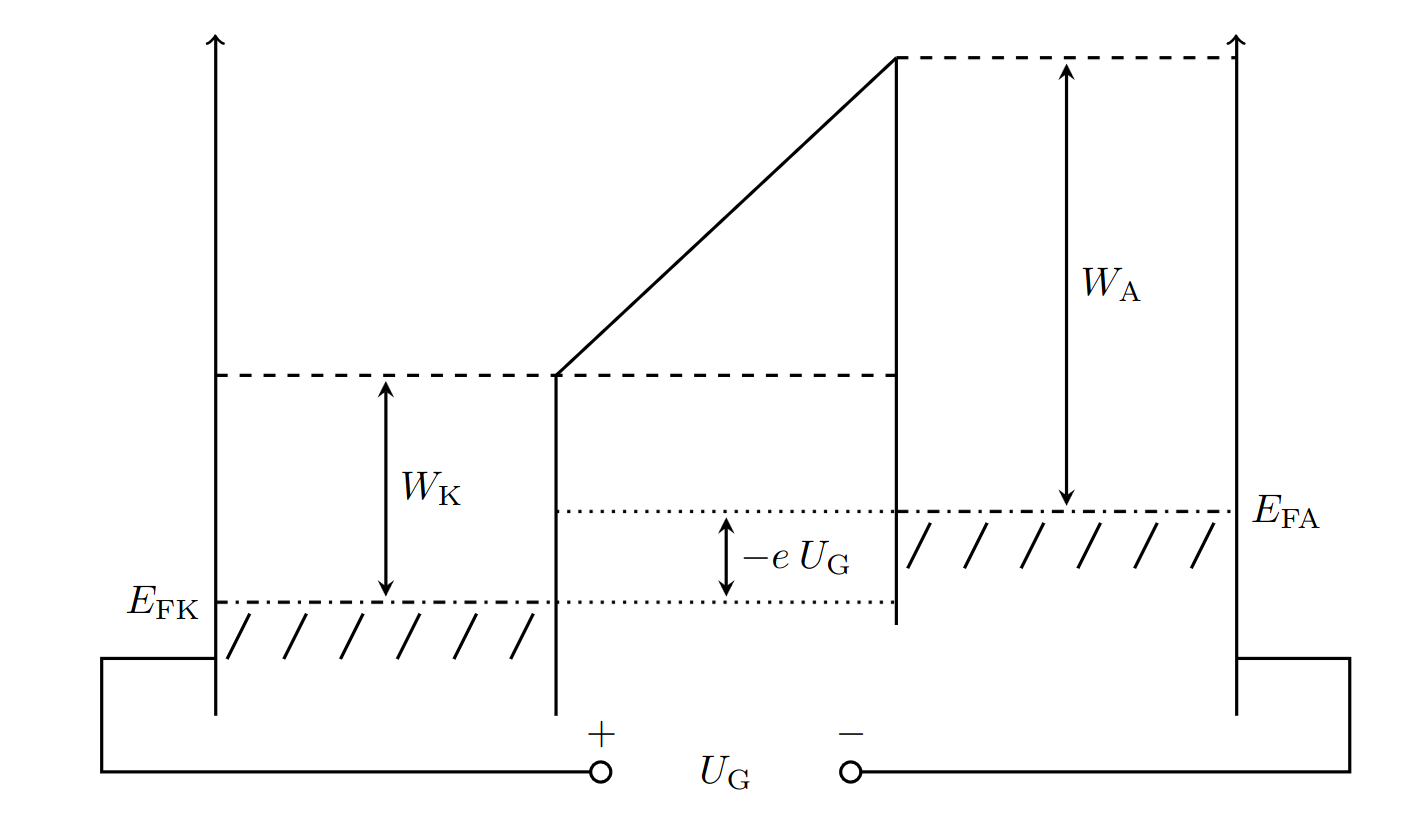
\includegraphics[width=.5\textwidth]{402_austrittsarbeit.png}
        \caption{Bänderschema der Anode und Kathode bei anlegen einer äußeren Spannung.\cite{Anleitung402}} \label{fig:bänderschema}
\end{figure}

\subsection{Experimenteller Aufbau}
Der experimentelle Aufbau ist in Abb.\ (\ref{fig:aufbau_photoeffekt}) zu sehen.
Die Hg--Lampe diente als Lichtquelle.
Mit der Blende und der Linse wurde die Intensität und Breite des Lichtstrahls so eingestellt, dass ein fokussierter Punkt auf der Photokathode zu sehen war.
Dabei wurde darauf geachtet, dass der Lichtstrahl nicht die Anode berührte.
Zur Vermeidung von Streulicht wurde über die Kathode--Anode--Anordnung eine Blende gestülpt, mit einem Rohrausschnitt, welcher auf das Filterrad zeigte.
Mit Hilfe des Filterrades wählte man verschiedene Wellenlängen zur Beobachtung aus.

Das Gegenfeld konnte mit einer separaten Spannung eingestellt und variiert werden.
Da die Spannnug, die für das Gegenfeld zur Verfügung stand, bis zu $\SI{12}{V}$ ausgeben kann, wurde diese mit einem Spannungsteiler auf $U'=\tfrac{R_1}{R_1+R_2}U=\tfrac{\SI{100}{\ohm}}{\SI{100}{\ohm}+\SI{333}{\ohm}}12V=\SI{2.77}{V}$ gedrosselt.
\begin{figure}[t]
        \centering
        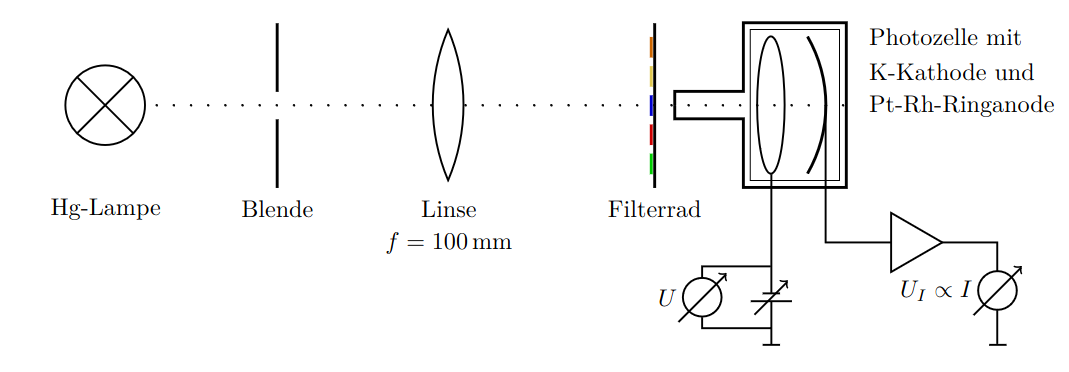
\includegraphics[width=.5\textwidth]{402_aufbau_photoeffekt.png}
        \caption{Experimenteller Aufbau zum Photoeffekt.} \label{fig:aufbau_photoeffekt}
\end{figure}

\subsection{Durchführung \& Auswertung}
Die Messung des Photostroms und des Gegenfeldes erfolgte über zwei DMMs.
Jede Messung wurde zwei mal durchgeführt und jeweils der Mittelwert verwendet, da die Intensität der Hg--Lampe schwankt.

Die Spannung des Gegenfeldes wurde für alle Interferenzfilter ($\SI{305}{nm}$, $\SI{365}{n m}$, $\SI{436}{n m}$, $\SI{546}{n m}$ und $\SI{578}{n m}$) von der maximalen Spannung ($\approx \SI{2.77}{V}$) bis zur minimalen Spannung $(\approx \SI{0.0006}{V}$) variiert und der Photostrom gemessen.
Der Anodenstrom $I_0$, der von der Anode zu Kathode fließt, wenn die Gegenspannung maximal ist, wurde jeweils gesondert gemessen, um diesen in der Auswertung von der Messung zu subtrahieren.

Bis zu einer gewissen Gegenfeldspannung $U_\text{G}=U_0$ fließt kein Photostrom $I$; ab $U_0$ fließt dieser mit einem quadratischen Zusammenhang zu $U_G$.

Für die Auswertung wird $\,\sqrt[]{I-I_0}$ -- der Photostrom $I$ abzüglich $I_0$ unter der Wurzel -- gegen die Gegenfeldspannung $U_G$ aufgetragen.
Die Graphen finden sich im Appendix von Abb.\ (\ref{fig:photo_auswertung_305}) bis Abb.\ (\ref{fig:photo_auswertung_578}).

Ein Geradenfit wird für alle Messdaten, die im quadratischen Bereich liegen durchgeführt.
Die Messpunkte, die kein quadratisches Verhalten zeigen, geben des Strom von der Anode zur Kathode an und werden nicht berücksichtigt.
$\chi ^2/\text{ddof}$ ist für alle Geraden viel kleiner als der ideale Wert 1.
Diese Diskrepanz ist hier nicht zu kleiner Fehler sondern einer Überfittung der Geraden zuzuordnen.
Die Nullstelle der Fitgeraden liefert genau den Wert der Gegenspannung, bei der kein Photostrom fließt.

\begin{table}[h]
        \begin{tabular}{cc}
                $\lambda $ & $U_0$ \\
                \hline
                $\SI{305}{n m}$ & $\SI{-1.1806+-0.0093}{V}$ \\
                $\SI{365}{n m}$ & $\SI{-1.509+-0.017}{V}$ \\
                $\SI{436}{n m}$ & $\SI{-0.951+-0.011}{V}$ \\
                $\SI{546}{n m}$ & $\SI{-0.2615+-0.0057}{V}$ \\
                $\SI{578}{n m}$ & $\SI{-0.388+-0.015}{V}$ 
        \end{tabular}
\end{table}
Trägt man diese Werte gegen die jeweilige Frequenz des Lichts auf, so lässt sich ein Geradenfit durchführen, dessen Steigung gleich dem \textsc{Planck}'schen Wirkungsquantum und dessen Achsenabschnitt gleich der Austrittsarbeit ist.
Dieser Plot ist in Abb.\ (\ref{fig:austrittsarbeit}) zu sehen.
$\chi ^2/\text{ddof}$ ist viel größer als 1, weil sich die Fehler, durch die kleinen Messfehler, in der Fehlerfortpflanzung minimiert haben.

\begin{figure}[t]
        \centering
        \resizebox{.5\textwidth}{!}{% GNUPLOT: LaTeX picture with Postscript
\begingroup
  \makeatletter
  \providecommand\color[2][]{%
    \GenericError{(gnuplot) \space\space\space\@spaces}{%
      Package color not loaded in conjunction with
      terminal option `colourtext'%
    }{See the gnuplot documentation for explanation.%
    }{Either use 'blacktext' in gnuplot or load the package
      color.sty in LaTeX.}%
    \renewcommand\color[2][]{}%
  }%
  \providecommand\includegraphics[2][]{%
    \GenericError{(gnuplot) \space\space\space\@spaces}{%
      Package graphicx or graphics not loaded%
    }{See the gnuplot documentation for explanation.%
    }{The gnuplot epslatex terminal needs graphicx.sty or graphics.sty.}%
    \renewcommand\includegraphics[2][]{}%
  }%
  \providecommand\rotatebox[2]{#2}%
  \@ifundefined{ifGPcolor}{%
    \newif\ifGPcolor
    \GPcolortrue
  }{}%
  \@ifundefined{ifGPblacktext}{%
    \newif\ifGPblacktext
    \GPblacktexttrue
  }{}%
  % define a \g@addto@macro without @ in the name:
  \let\gplgaddtomacro\g@addto@macro
  % define empty templates for all commands taking text:
  \gdef\gplbacktext{}%
  \gdef\gplfronttext{}%
  \makeatother
  \ifGPblacktext
    % no textcolor at all
    \def\colorrgb#1{}%
    \def\colorgray#1{}%
  \else
    % gray or color?
    \ifGPcolor
      \def\colorrgb#1{\color[rgb]{#1}}%
      \def\colorgray#1{\color[gray]{#1}}%
      \expandafter\def\csname LTw\endcsname{\color{white}}%
      \expandafter\def\csname LTb\endcsname{\color{black}}%
      \expandafter\def\csname LTa\endcsname{\color{black}}%
      \expandafter\def\csname LT0\endcsname{\color[rgb]{1,0,0}}%
      \expandafter\def\csname LT1\endcsname{\color[rgb]{0,1,0}}%
      \expandafter\def\csname LT2\endcsname{\color[rgb]{0,0,1}}%
      \expandafter\def\csname LT3\endcsname{\color[rgb]{1,0,1}}%
      \expandafter\def\csname LT4\endcsname{\color[rgb]{0,1,1}}%
      \expandafter\def\csname LT5\endcsname{\color[rgb]{1,1,0}}%
      \expandafter\def\csname LT6\endcsname{\color[rgb]{0,0,0}}%
      \expandafter\def\csname LT7\endcsname{\color[rgb]{1,0.3,0}}%
      \expandafter\def\csname LT8\endcsname{\color[rgb]{0.5,0.5,0.5}}%
    \else
      % gray
      \def\colorrgb#1{\color{black}}%
      \def\colorgray#1{\color[gray]{#1}}%
      \expandafter\def\csname LTw\endcsname{\color{white}}%
      \expandafter\def\csname LTb\endcsname{\color{black}}%
      \expandafter\def\csname LTa\endcsname{\color{black}}%
      \expandafter\def\csname LT0\endcsname{\color{black}}%
      \expandafter\def\csname LT1\endcsname{\color{black}}%
      \expandafter\def\csname LT2\endcsname{\color{black}}%
      \expandafter\def\csname LT3\endcsname{\color{black}}%
      \expandafter\def\csname LT4\endcsname{\color{black}}%
      \expandafter\def\csname LT5\endcsname{\color{black}}%
      \expandafter\def\csname LT6\endcsname{\color{black}}%
      \expandafter\def\csname LT7\endcsname{\color{black}}%
      \expandafter\def\csname LT8\endcsname{\color{black}}%
    \fi
  \fi
    \setlength{\unitlength}{0.0500bp}%
    \ifx\gptboxheight\undefined%
      \newlength{\gptboxheight}%
      \newlength{\gptboxwidth}%
      \newsavebox{\gptboxtext}%
    \fi%
    \setlength{\fboxrule}{0.5pt}%
    \setlength{\fboxsep}{1pt}%
    \definecolor{tbcol}{rgb}{1,1,1}%
\begin{picture}(7200.00,4320.00)%
    \gplgaddtomacro\gplbacktext{%
      \csname LTb\endcsname%%
      \put(634,619){\makebox(0,0)[r]{\strut{}$0.2$}}%
      \csname LTb\endcsname%%
      \put(634,1062){\makebox(0,0)[r]{\strut{}$0.4$}}%
      \csname LTb\endcsname%%
      \put(634,1505){\makebox(0,0)[r]{\strut{}$0.6$}}%
      \csname LTb\endcsname%%
      \put(634,1947){\makebox(0,0)[r]{\strut{}$0.8$}}%
      \csname LTb\endcsname%%
      \put(634,2390){\makebox(0,0)[r]{\strut{}$1$}}%
      \csname LTb\endcsname%%
      \put(634,2833){\makebox(0,0)[r]{\strut{}$1.2$}}%
      \csname LTb\endcsname%%
      \put(634,3276){\makebox(0,0)[r]{\strut{}$1.4$}}%
      \csname LTb\endcsname%%
      \put(634,3719){\makebox(0,0)[r]{\strut{}$1.6$}}%
      \csname LTb\endcsname%%
      \put(731,425){\makebox(0,0){\strut{}$5$}}%
      \csname LTb\endcsname%%
      \put(1347,425){\makebox(0,0){\strut{}$5.5$}}%
      \csname LTb\endcsname%%
      \put(1962,425){\makebox(0,0){\strut{}$6$}}%
      \csname LTb\endcsname%%
      \put(2578,425){\makebox(0,0){\strut{}$6.5$}}%
      \csname LTb\endcsname%%
      \put(3193,425){\makebox(0,0){\strut{}$7$}}%
      \csname LTb\endcsname%%
      \put(3809,425){\makebox(0,0){\strut{}$7.5$}}%
      \csname LTb\endcsname%%
      \put(4424,425){\makebox(0,0){\strut{}$8$}}%
      \csname LTb\endcsname%%
      \put(5039,425){\makebox(0,0){\strut{}$8.5$}}%
      \csname LTb\endcsname%%
      \put(5655,425){\makebox(0,0){\strut{}$9$}}%
      \csname LTb\endcsname%%
      \put(6270,425){\makebox(0,0){\strut{}$9.5$}}%
      \csname LTb\endcsname%%
      \put(6886,425){\makebox(0,0){\strut{}$10$}}%
    }%
    \gplgaddtomacro\gplfronttext{%
      \csname LTb\endcsname%%
      \put(170,2169){\rotatebox{-270}{\makebox(0,0){\strut{}$U_0/\SI{}{V}$}}}%
      \csname LTb\endcsname%%
      \put(3809,135){\makebox(0,0){\strut{}$\nu / \SI{}{10^{14} Hz}$}}%
      \csname LTb\endcsname%%
      \put(6123,1083){\makebox(0,0)[r]{\strut{}$U_0$ Datenpunkte}}%
      \csname LTb\endcsname%%
      \put(6123,890){\makebox(0,0)[r]{\strut{}$f(\nu)=\SI{0.228 +- 0.065}{V/\ 10^{14} Hz}\cdot \nu \SI{-0.90 +- 0.45}{V}$}}%
      \csname LTb\endcsname%%
      \put(3809,4009){\makebox(0,0){\strut{}$W_A=\SI{-0.90 +- 0.45}{eV}$, $\text{h}=\SI{0.0228 +- 0.0065 }{eVs} \cdot 10^{-15} $ und $\chi^2/\text{ddof}=752.338$}}%
    }%
    \gplbacktext
    \put(0,0){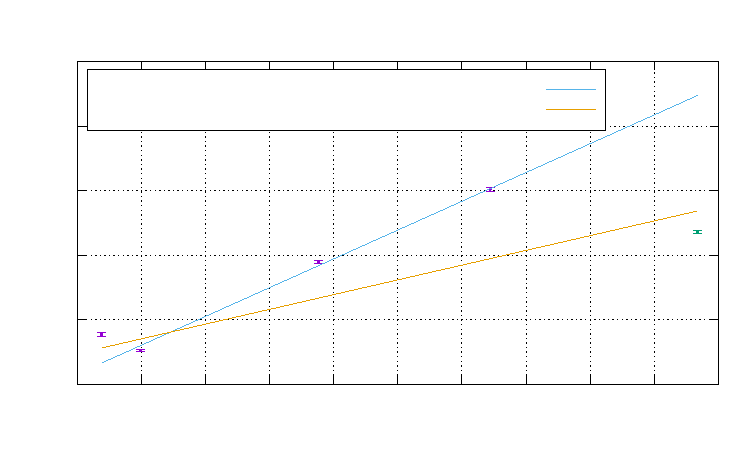
\includegraphics[width={360.00bp},height={216.00bp}]{Austrittsarbeit}}%
    \gplfronttext
  \end{picture}%
\endgroup
}
        \caption{Gemessene Gegenspannung $U_0$ gegen die Frequenz der auf die Kathode treffenden Photonen. Der Achsenabschnitt ist $W_\text{A}$ und die Steigung ist $h$.} \label{fig:austrittsarbeit}
\end{figure}
Es ergibt sich ein Wert von
\begin{align} 
        h=\SI{4.46+-0.64e-15}{eVs}
.\end{align} 
Der aktuelle CODATA\cite{CODATA} Wert ist
\begin{align} 
        h_\text{CODATA}\approx \SI{4.136e-15}{eVs}
.\end{align} 
Die Abweichung des gemessenen Werts liegt bei ca.\ $8\%$.
Dieser Wert liegt unter $10\%$ Abweichung, was aufgrund der passenden Geradenfits und guten Messwerte erwartet war.
Geringe Abweichung können sich auch durch das relativ hohes $\chi ^2/\text{ddof}$ ergeben haben.

Die Austrittsarbeit wurde bestimmt zu
\begin{align} 
        W_\text{A}=\SI{-2.15+-0.38}{eV}
.\end{align} 
Aus \cite{LeyboldPhotoeffekt} lässt sich entnehmen, dass die Anode aus Platin besteht, welche eine Austrittsarbeit von 
\begin{align} 
        W_\text{lit.}=\SI{-5.32}{eV}
\end{align} 
bestitzt.
Der Wert ist \cite{SpektrumPhysik} entnommen.
Die Abweichung liegt bei $60\%$.
Dies war nicht erwartet, da die Abweichung von $h$ vom Literaturwert sehr gering ist.
Es ist allerdings nicht klar, ob die Anode vollständig aus Platin besteht, oder ein Gemisch aus Platin und anderen Materialien ist bzw.\ noch eine Legierung besitzt.
Wäre das der Fall, dann wäre die Abweichung verständlich.

Die Intensität des Lichtstrahl in der Theorie keine Auswirkung auf die kinetische Energie der Elektronen, also auch auf die Gegenspannung, da die Energie der Photonen nur abhängig von der Wellenlänge ist.
Die Erwartung ist also keine Abweichung der Gegenspannung.

Zur Kontrolle wurde für die Wellenlänge $\SI{365}{\nano m}$ eine Messung mit höherer Intensität durchgeführt.
Das Ergebnis ist in Abb.\ (\ref{fig:photostrom_hohe_intensität}) zu sehen.
Es ergibt sich eine Gegenspannung von $U_0^h=-\SI{1.87+-.1}{V}$.
Die Gegenspannung bei niedriger Intensität liegt bei $U_0^n=\SI{-1.509+-.017}{V}$.
Das entspricht einer Abweichung von $U_0^h$ von $U_0^n$ von ca.\ $24\%$.
Diese Abweichung entspricht nicht der Erwartung.
Eine Abweichung ist hier allerdings keine Anfechtung der Theorie, sondern eine ungenaue Messung.
Die Fitgerade für die Datenpunkte bei hoher Intensität hat eine Güte von $\chi ^2/\text{ddof}\approx 21$, was für einen passenden Geradenfit zu hoch ist.
Die Fehler der Messdaten wurden hier zu klein gewählt, was zu Abweichungen der Nullstelle der Geraden geführt hat.

\begin{figure}[t]
        \centering
        \resizebox{.5\textwidth}{!}{% GNUPLOT: LaTeX picture with Postscript
\documentclass{minimal}
% Set font size
\makeatletter
\def\@ptsize{1}
\InputIfFileExists{size11.clo}{}{%
   \GenericError{(gnuplot) \space\space\space\@spaces}{%
      Gnuplot Error: File `size11.clo' not found! Could not set font size%
   }{See the gnuplot documentation for explanation.%
   }{For using a font size a file `size<fontsize>.clo' has to exist.
        Falling back ^^Jto default fontsize 10pt.}%
  \def\@ptsize{0}
  \input{size10.clo}%
}%
\makeatother
% Load packages
\usepackage{calc}
\usepackage{graphicx}
\usepackage{color}
\usepackage{transparent}
\makeatletter
% Select an appropriate default driver (from TeXLive graphics.cfg)
\begingroup
  \chardef\x=0 %
  % check pdfTeX
  \@ifundefined{pdfoutput}{}{%
    \ifcase\pdfoutput
    \else
      \chardef\x=1 %
    \fi
  }%
  % check VTeX
  \@ifundefined{OpMode}{}{%
    \chardef\x=2 %
  }%
\expandafter\endgroup
\ifcase\x
  % default case
  \PassOptionsToPackage{dvips}{geometry}
\or
  % pdfTeX is running in pdf mode
  \PassOptionsToPackage{pdftex}{geometry}
\else
  % VTeX is running
  \PassOptionsToPackage{vtex}{geometry}
\fi
\makeatother
% Set papersize
\usepackage[papersize={360.00bp,216.00bp},text={360.00bp,216.00bp}]{geometry}
% No page numbers and no paragraph indentation
\pagestyle{empty}
\setlength{\parindent}{0bp}%
% Load configuration file
\InputIfFileExists{gnuplot.cfg}{%
  \typeout{Using configuration file gnuplot.cfg}%
}{%
 \typeout{No configuration file gnuplot.cfg found.}%
}%
\usepackage{siunitx}
\begin{document}
\begingroup
  \makeatletter
  \providecommand\color[2][]{%
    \GenericError{(gnuplot) \space\space\space\@spaces}{%
      Package color not loaded in conjunction with
      terminal option `colourtext'%
    }{See the gnuplot documentation for explanation.%
    }{Either use 'blacktext' in gnuplot or load the package
      color.sty in LaTeX.}%
    \renewcommand\color[2][]{}%
  }%
  \providecommand\includegraphics[2][]{%
    \GenericError{(gnuplot) \space\space\space\@spaces}{%
      Package graphicx or graphics not loaded%
    }{See the gnuplot documentation for explanation.%
    }{The gnuplot epslatex terminal needs graphicx.sty or graphics.sty.}%
    \renewcommand\includegraphics[2][]{}%
  }%
  \providecommand\rotatebox[2]{#2}%
  \@ifundefined{ifGPcolor}{%
    \newif\ifGPcolor
    \GPcolortrue
  }{}%
  \@ifundefined{ifGPblacktext}{%
    \newif\ifGPblacktext
    \GPblacktexttrue
  }{}%
  % define a \g@addto@macro without @ in the name:
  \let\gplgaddtomacro\g@addto@macro
  % define empty templates for all commands taking text:
  \gdef\gplbacktext{}%
  \gdef\gplfronttext{}%
  \makeatother
  \ifGPblacktext
    % no textcolor at all
    \def\colorrgb#1{}%
    \def\colorgray#1{}%
  \else
    % gray or color?
    \ifGPcolor
      \def\colorrgb#1{\color[rgb]{#1}}%
      \def\colorgray#1{\color[gray]{#1}}%
      \expandafter\def\csname LTw\endcsname{\color{white}}%
      \expandafter\def\csname LTb\endcsname{\color{black}}%
      \expandafter\def\csname LTa\endcsname{\color{black}}%
      \expandafter\def\csname LT0\endcsname{\color[rgb]{1,0,0}}%
      \expandafter\def\csname LT1\endcsname{\color[rgb]{0,1,0}}%
      \expandafter\def\csname LT2\endcsname{\color[rgb]{0,0,1}}%
      \expandafter\def\csname LT3\endcsname{\color[rgb]{1,0,1}}%
      \expandafter\def\csname LT4\endcsname{\color[rgb]{0,1,1}}%
      \expandafter\def\csname LT5\endcsname{\color[rgb]{1,1,0}}%
      \expandafter\def\csname LT6\endcsname{\color[rgb]{0,0,0}}%
      \expandafter\def\csname LT7\endcsname{\color[rgb]{1,0.3,0}}%
      \expandafter\def\csname LT8\endcsname{\color[rgb]{0.5,0.5,0.5}}%
    \else
      % gray
      \def\colorrgb#1{\color{black}}%
      \def\colorgray#1{\color[gray]{#1}}%
      \expandafter\def\csname LTw\endcsname{\color{white}}%
      \expandafter\def\csname LTb\endcsname{\color{black}}%
      \expandafter\def\csname LTa\endcsname{\color{black}}%
      \expandafter\def\csname LT0\endcsname{\color{black}}%
      \expandafter\def\csname LT1\endcsname{\color{black}}%
      \expandafter\def\csname LT2\endcsname{\color{black}}%
      \expandafter\def\csname LT3\endcsname{\color{black}}%
      \expandafter\def\csname LT4\endcsname{\color{black}}%
      \expandafter\def\csname LT5\endcsname{\color{black}}%
      \expandafter\def\csname LT6\endcsname{\color{black}}%
      \expandafter\def\csname LT7\endcsname{\color{black}}%
      \expandafter\def\csname LT8\endcsname{\color{black}}%
    \fi
  \fi
    \setlength{\unitlength}{0.0500bp}%
    \ifx\gptboxheight\undefined%
      \newlength{\gptboxheight}%
      \newlength{\gptboxwidth}%
      \newsavebox{\gptboxtext}%
    \fi%
    \setlength{\fboxrule}{0.5pt}%
    \setlength{\fboxsep}{1pt}%
    \definecolor{tbcol}{rgb}{1,1,1}%
\begin{picture}(7200.00,4320.00)%
    \gplgaddtomacro\gplbacktext{%
      \csname LTb\endcsname%%
      \put(634,619){\makebox(0,0)[r]{\strut{}$-10$}}%
      \csname LTb\endcsname%%
      \put(634,963){\makebox(0,0)[r]{\strut{}$0$}}%
      \csname LTb\endcsname%%
      \put(634,1308){\makebox(0,0)[r]{\strut{}$10$}}%
      \csname LTb\endcsname%%
      \put(634,1652){\makebox(0,0)[r]{\strut{}$20$}}%
      \csname LTb\endcsname%%
      \put(634,1997){\makebox(0,0)[r]{\strut{}$30$}}%
      \csname LTb\endcsname%%
      \put(634,2341){\makebox(0,0)[r]{\strut{}$40$}}%
      \csname LTb\endcsname%%
      \put(634,2686){\makebox(0,0)[r]{\strut{}$50$}}%
      \csname LTb\endcsname%%
      \put(634,3030){\makebox(0,0)[r]{\strut{}$60$}}%
      \csname LTb\endcsname%%
      \put(634,3374){\makebox(0,0)[r]{\strut{}$70$}}%
      \csname LTb\endcsname%%
      \put(634,3719){\makebox(0,0)[r]{\strut{}$80$}}%
      \csname LTb\endcsname%%
      \put(731,425){\makebox(0,0){\strut{}$-2.5$}}%
      \csname LTb\endcsname%%
      \put(1915,425){\makebox(0,0){\strut{}$-2$}}%
      \csname LTb\endcsname%%
      \put(3098,425){\makebox(0,0){\strut{}$-1.5$}}%
      \csname LTb\endcsname%%
      \put(4282,425){\makebox(0,0){\strut{}$-1$}}%
      \csname LTb\endcsname%%
      \put(5466,425){\makebox(0,0){\strut{}$-0.5$}}%
      \csname LTb\endcsname%%
      \put(6649,425){\makebox(0,0){\strut{}$0$}}%
    }%
    \gplgaddtomacro\gplfronttext{%
      \csname LTb\endcsname%%
      \put(4158,3448){\makebox(0,0)[r]{\strut{}quadratische Datenpunkte}}%
      \csname LTb\endcsname%%
      \put(4158,3255){\makebox(0,0)[r]{\strut{}nicht quadratische Datenpunkte}}%
      \csname LTb\endcsname%%
      \put(4158,3061){\makebox(0,0)[r]{\strut{}$f(U_G)=\SI{40.4 +- 1.9}{}\cdot U_G + \SI{75.5 +- 2.2}{\milli V}$}}%
      \csname LTb\endcsname%%
      \put(170,2169){\rotatebox{-270.00}{\makebox(0,0){\strut{}$\sqrt{I-I_0}$/mV}}}%
      \csname LTb\endcsname%%
      \put(3809,135){\makebox(0,0){\strut{}$U_G$/V}}%
      \csname LTb\endcsname%%
      \put(3809,4009){\makebox(0,0){\strut{}$\lambda=\SI{365}{\nano m}$(GB): $U_0=\SI{-1.87 +- 0.10}{V}$ und $\chi^2/\text{ddof}=\SI{21.290}{}$}}%
    }%
    \gplbacktext
    \put(0,0){\includegraphics[width={360.00bp},height={216.00bp}]{365nmGB-inc}}%
    \gplfronttext
  \end{picture}%
\endgroup
\end{document}
}
        \caption{Photostrom abzüglich des Anodenstroms gegen Gegenspannung für $\lambda =\SI{365}{n m}$. Fit nur an Messdaten quadratisch ab $U_0$ und in quadratischer Abhängigkeit. Höhere Intensität als bei allen anderen Plots zum Photostrom.} \label{fig:photostrom_hohe_intensität}
\end{figure}

\section{\textsc{Balmer}--Serie}
Mit Hilfe der \textsc{Balmer}--Serie wird die Gitterkonstante des verwendeten Refelxionsgitters berechnet und die Breite der Isotopieaufspaltung bestimmt.
Es wird die \textsc{Rydberg}--Konstante $R$ und daraus das \textsc{Planck}'sche Wirkungsquantum $h$ bestimmt.

\subsection{Theoretischer Hintergrund: Gitterkonstante \& Interferenz}
Trifft ein einlaufender Strahl $i$ kohärenten Lichts im Winkel $\varphi _i$ auf ein Stufengitter wie in Abb.\ (\ref{fig:blazegitter}), so kommt es zu Interferenz zwischen allen im Winkel $\varphi _f$ auslaufenden Strahlen $f$.
Diese Interferenzmaxima kommen durch den Gangunterschied $\Delta $ zwischen dem einlaufende und auslaufenden Strahl zustande.
Dieser berechnet sich separat für beide Strahlen zu $\Delta =\Delta _i+\Delta _f=g\left(\sin \varphi _i+\sin \varphi _f\right)=g\left(\sin \alpha +\sin \beta \right)$.
Die Winkel $\alpha $ und $\beta $ sind identisch mit den Winkeln $\alpha $ und $\beta $ aus Abb.\ (\ref{fig:blazegitter}).
$g$ ist die Gitterkonstante.

Ein Interferenzmaximum entsteht durch eine Überlagerung von Wellen, die um Vielfache ihrer Wellenlänge, $n \lambda $, voneinander verschoben sind.

Die Interferenzmaxima verhalten sich also in Abhängigkeit der Wellenlänge wie
\begin{align} 
        n \lambda =g\left(\sin \alpha +\sin \beta \right)=\Delta 
.\end{align} 
\begin{figure}[t]
        \centering
        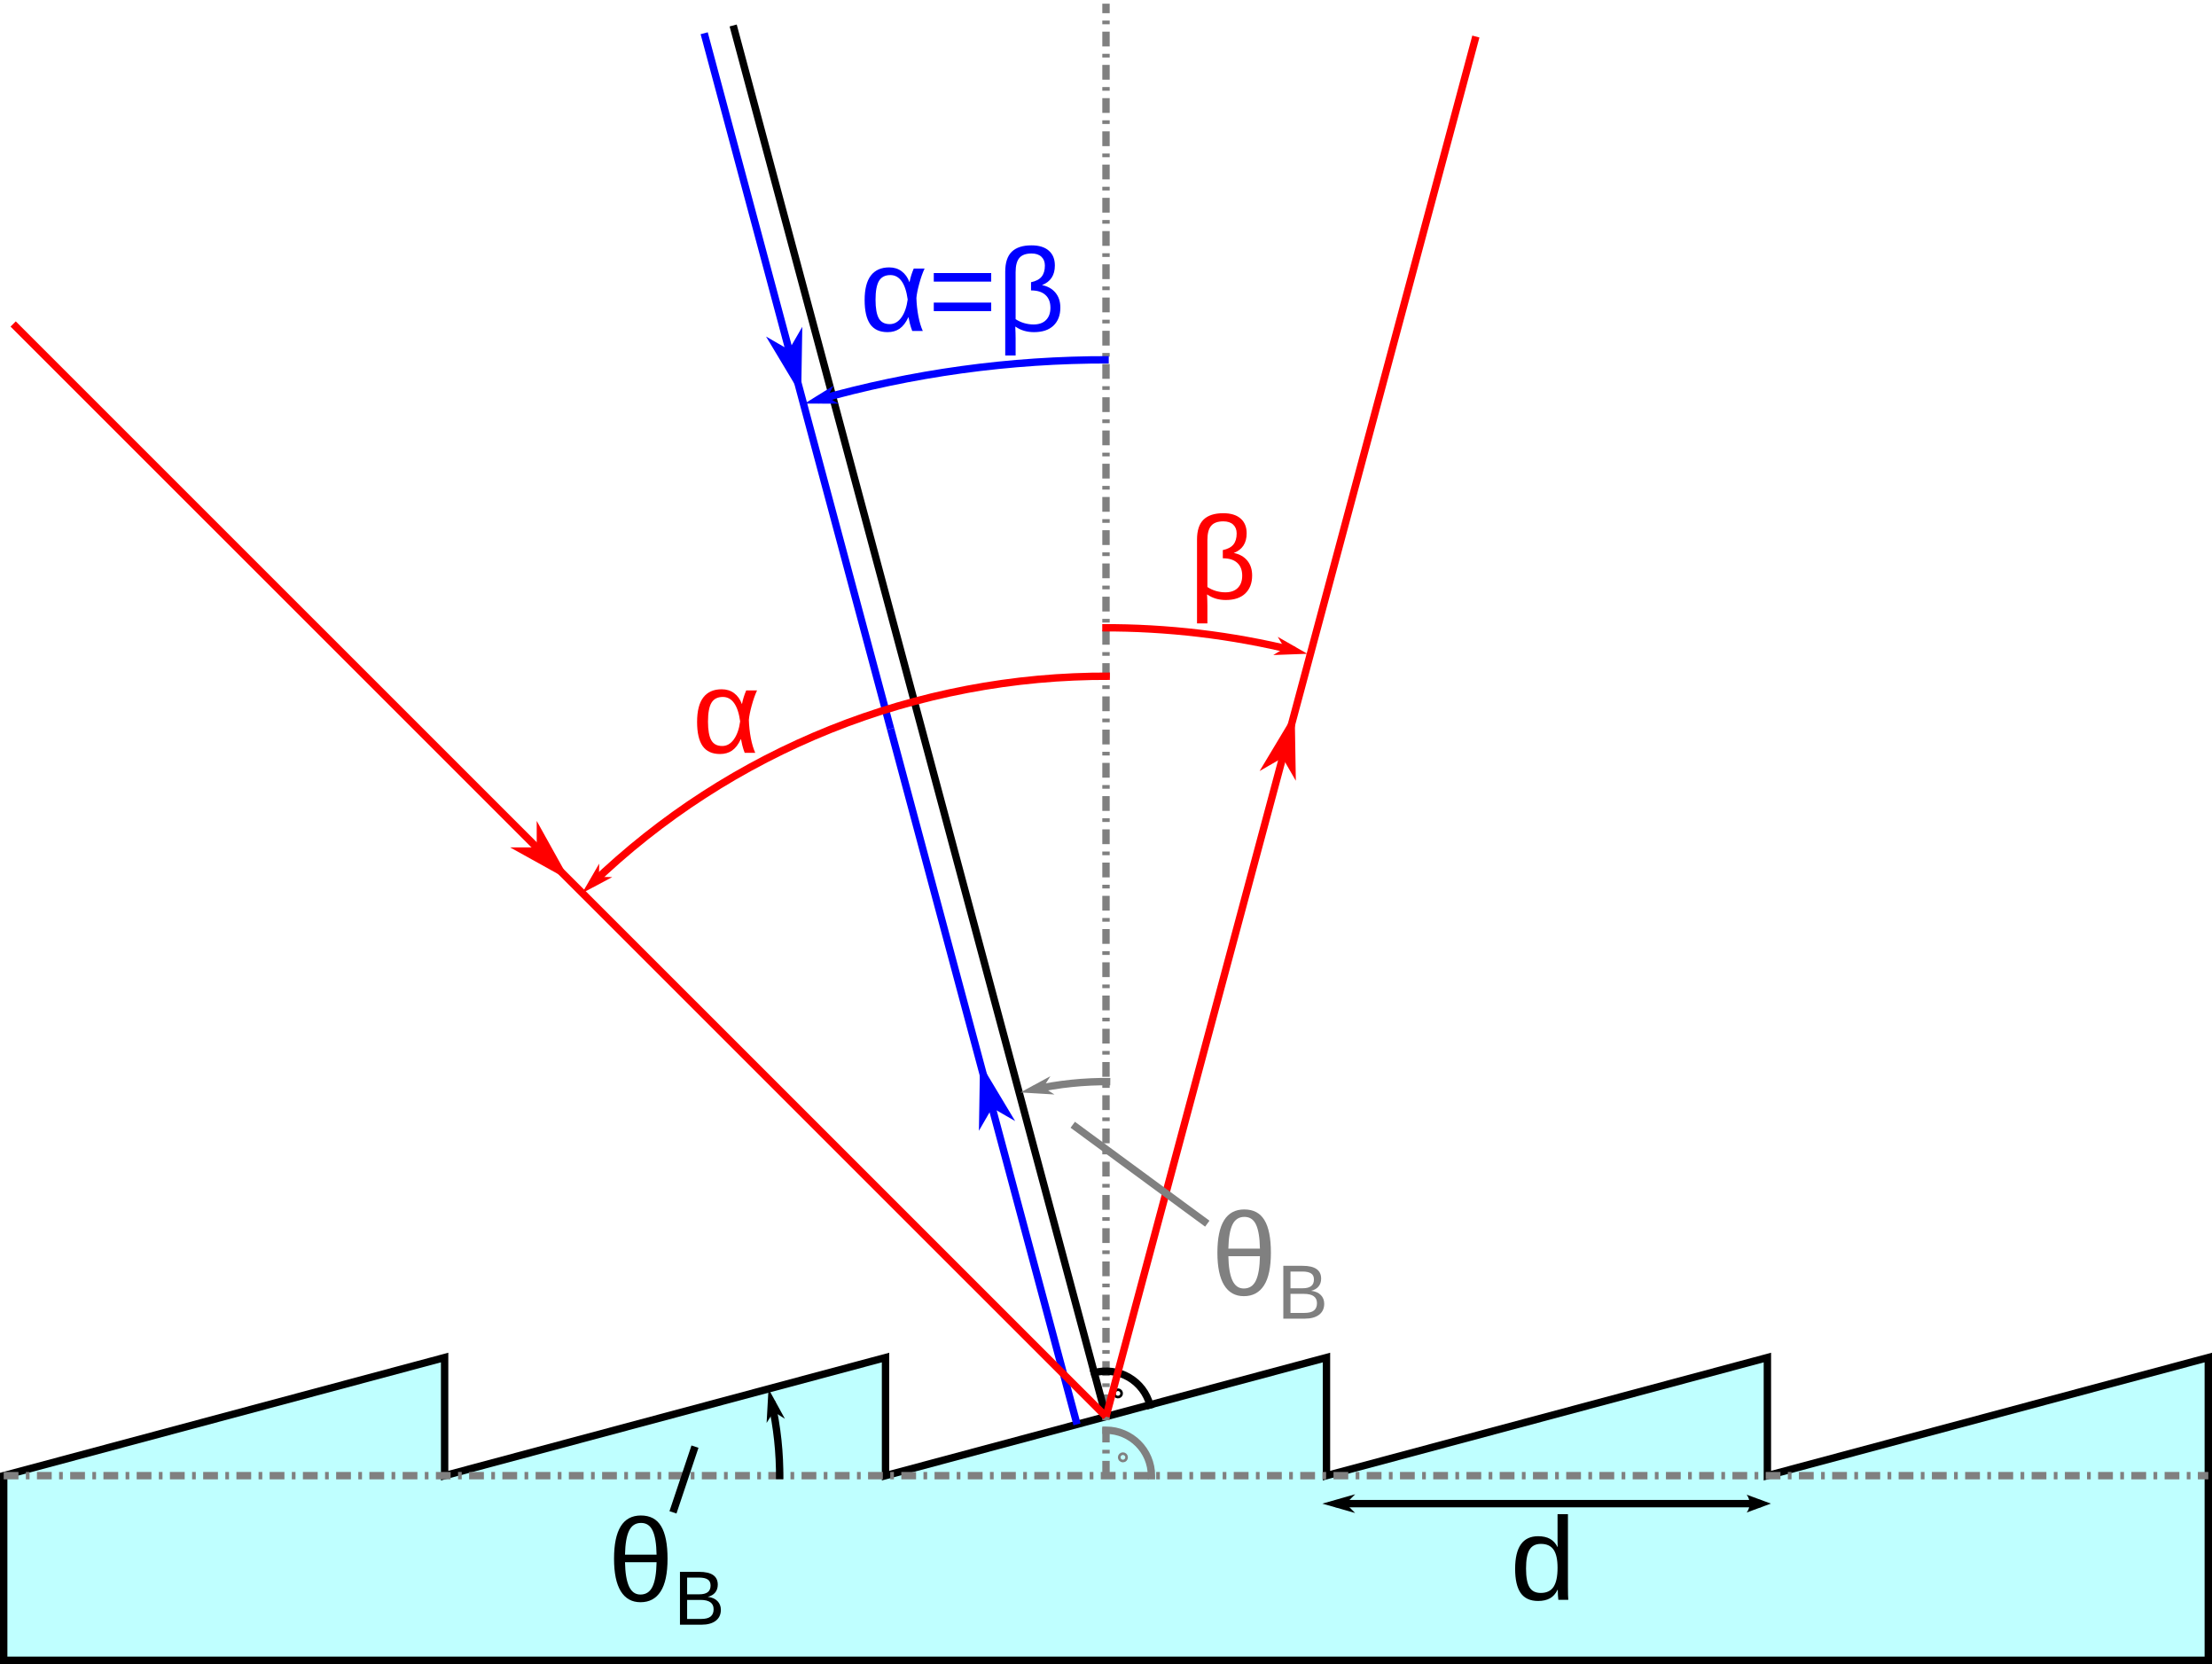
\includegraphics[width=.5\textwidth]{402_stufengitter.png}
        \caption{Schematische Darstellung des im Versuch verwendeten Gitters. Hier in der \textsc{Littrow}--Anordnung.\cite{WikipediaBlazegitter}} \label{fig:blazegitter}
\end{figure}

\subsection{Theoretischer Hintergrund: Spektrallinien}
\subsubsection{Energieniveaus \& Spektrallinien}
Diskrete Spektrallinien lassen sich aufgrund der Quantelung von Energie verstehen.
Im Orbitalmodell ist es Elektronen möglich diese gequantelte Energie in Form eines Photons aufzunehmen und abzugeben.
Dabei ändert es für jeden Übergang seinen Zustand (Energieniveau) beschrieben durch die Hauptquantenzahl $n$.
Die Energie in Abhängigkeit des Niveaus ist beschrieben durch $E_n=-\tfrac{\SI{13.6}{eV}}{n^2}$.
Der Energieunterschied zwischen zwei Niveaus kann mit der \textsc{Rydberg}--Formel für Wasserstoffähnliche Atome als 
\begin{align} 
        E_{n_<,n_>}=hcRZ^2\left(\dfrac{1}{n_<^2}-\dfrac{1}{n_>^2}\right)=\dfrac{hc}{\lambda _\text{vac}}
\end{align} 
geschrieben werden.
Hier ist $n_<$ das niedrigere Niveau und $n_>$ das höhere Niveau, $Z$ die Protonenzahl und $R$ die \textsc{Rydberg}--Konstante für das jeweilige Atom.

Für Wasserstoff lässt sich aus Leybold Didactic \cite{LeyboldBalmerserieBeobachtung} folgende Formel entnehmen (diese wird für die Auswertung verwendet):
\begin{align} 
        R_\text{H}=\mu R_{\infty}=\mu \dfrac{m_e e^4}{8\varepsilon _0^2h^3c}
,\end{align} 
mit $R_\text{H}$ der spezifischen \textsc{Rydberg}--Konstante für Wasserstoff und $\mu =\tfrac{m_em_K}{m_e+m_K}$ der reduzierten Masse.
Der Zusammenhang mit der Energie ist
\begin{align} 
        E_{n_<,n_>}=hR_\infty\left(\dfrac{1}{n_<^2}-\dfrac{1}{n_>^2}\right)=h\nu 
,\end{align} 
mit $\nu $ der Wellenlänge des emittierten Photons aus Wasserstoff.

Für ausgezeichente Übergänge wird eine Namenskonvention eingeführt.
Alle Übergänge auf $n_<=1$ werden \textsc{Lyman} genannt; auf $n_<=2$ \textsc{Balmer}; auf $n_<=3$ \textsc{Paschen}; etc.\ .
Diese Übergänge werden weiter verfeinert in $n_>=n_<+i$ mit $i=1\equiv \alpha $, $i=2\equiv \beta $, $i=3\equiv \gamma $, etc.\ .
Diese Konvention ist in Abb.\ (\ref{fig:serien}) dargestellt.
Die \textsc{Balmer} Übergange sind insofern besonders, als dass sie im sichtbaren Spektrum liegen.

\begin{figure}[t]
        \centering
        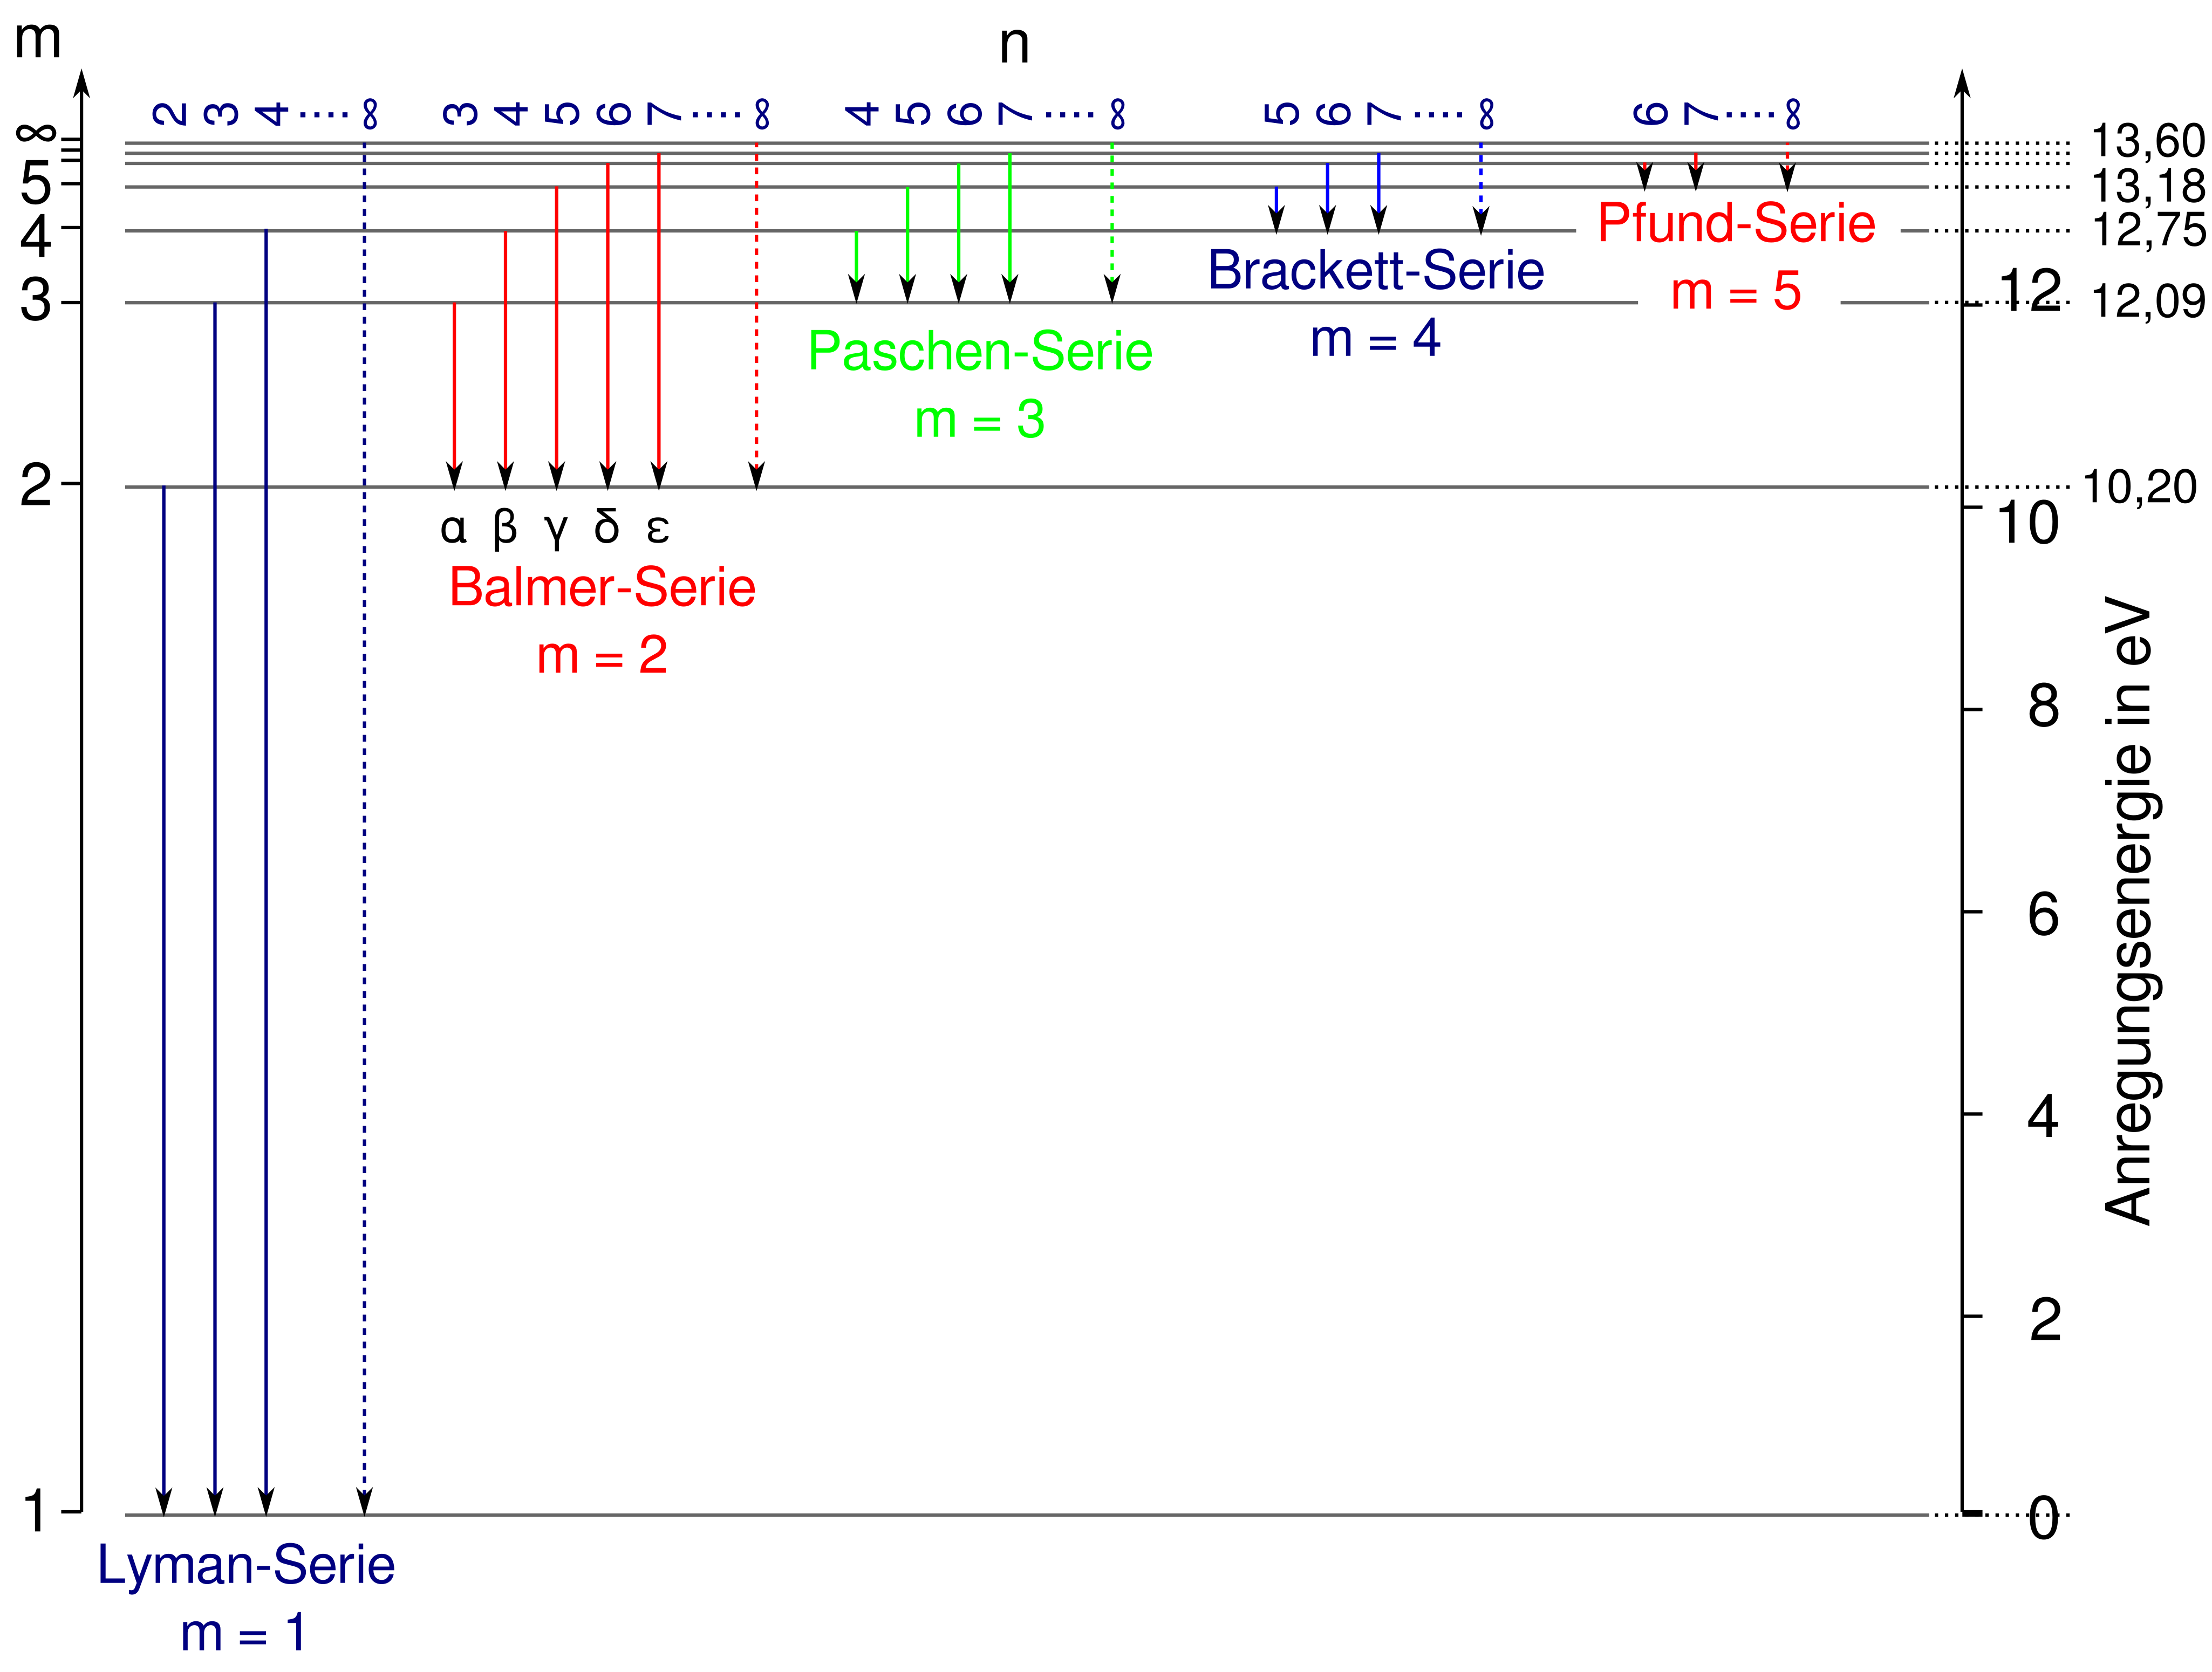
\includegraphics[width=.5\textwidth]{402_serien.png}
        \caption{Energieniveaus des Wasserstoffs mit benannten Serien (Übergängen).\cite{WikipediaSerien}} \label{fig:serien}
\end{figure}

\subsubsection{Linienverbreiterung \& Isotopieaufspaltung}
Spektrallinien sind nicht exakt einer Wellenlänge zuzuordnen, da sie eine gewisse Linienbreite besitzen.
Die natürliche Linienbreite $\Gamma $ ist auf die quantenmechanische Unschärferelation $\Delta _E\Delta _t \geq \tfrac{\hbar }{2}$ zurückzuführen.
Sie verhält sich wie $\Gamma \tau =\hbar $, mit $\tau =\tfrac{1}{\lambda }$ der Lebensdauer des Zustands und $\lambda $ der Zerfallskonstante.

Es kann zur Linienverbreiterung durch den \textsc{Doppler}--Effekt kommen.
In Abhängigkeit davon, wie schnell sich die Atome im Gas bewegen, sind ihre Energieniveaus \textsc{Doppler}--verschoben was dazu führt, dass Photonen emittiert werden, die eine Verteilung um die theoretisch exakte Wellenlänge der Spektrallinie besitzen.

Isotope eines Elements besitzen aufgrund gleicher Protonenzahl aber verschiedener Neutronenzahl eine unterschiedliche Masse.
Dieser Massenunterschied führt dazu, dass die Spektrallinien eines Elements von denen ihrer Isotope verschoben sind.
Die Größe der Aufspaltung berechnet sich mit 
\begin{align} 
         &&&& \partial _\beta \lambda  &= \partial _\beta\dfrac{g}{n}\left(\sin \alpha +\sin \beta \right)  &&&& \\
          &&&&  &= \dfrac{g}{n}\beta \cos \beta .  &&&& 
\end{align} 
Näherungsweise gilt dann die Formel
\begin{align} 
        \Delta \lambda =\dfrac{g}{n}\Delta \beta \cos \beta
,\end{align} 
mit $\Delta \beta =\tfrac{d}{f}$, wobei $d$ der Abstand der Linien und $f$ die Brennweite des Okulars ist.

\subsection{Experimenteller Aufbau}
Der experimentelle Aufbau ist in Abb.\ (\ref{fig:aufbau_spektrallinie}) zu sehen.
a ist die Gasentladungslampe (Hg--Lampe, oder \textsc{Balmer}--Lampe mit einem Anteil Deuterium); b der Abbildespalt um möglichst scharfe Linien zu erzeugen; c eine Linse die auf das Objektiv d fokussiert, um ein paralleles Strahlenbündel auf das Reflexionsgitter e zu richten; f eine Linse, die die auslaufenden paralellen Strahlen des Gitters auf das Objektiv g oder die CCD h fokussiert.

Alle optischen Bauteile werden so justiert, dass am Objektiv oder der CCD eine scharfe Spektrallinie zu erkennen ist.
\begin{figure}[t]
        \centering
        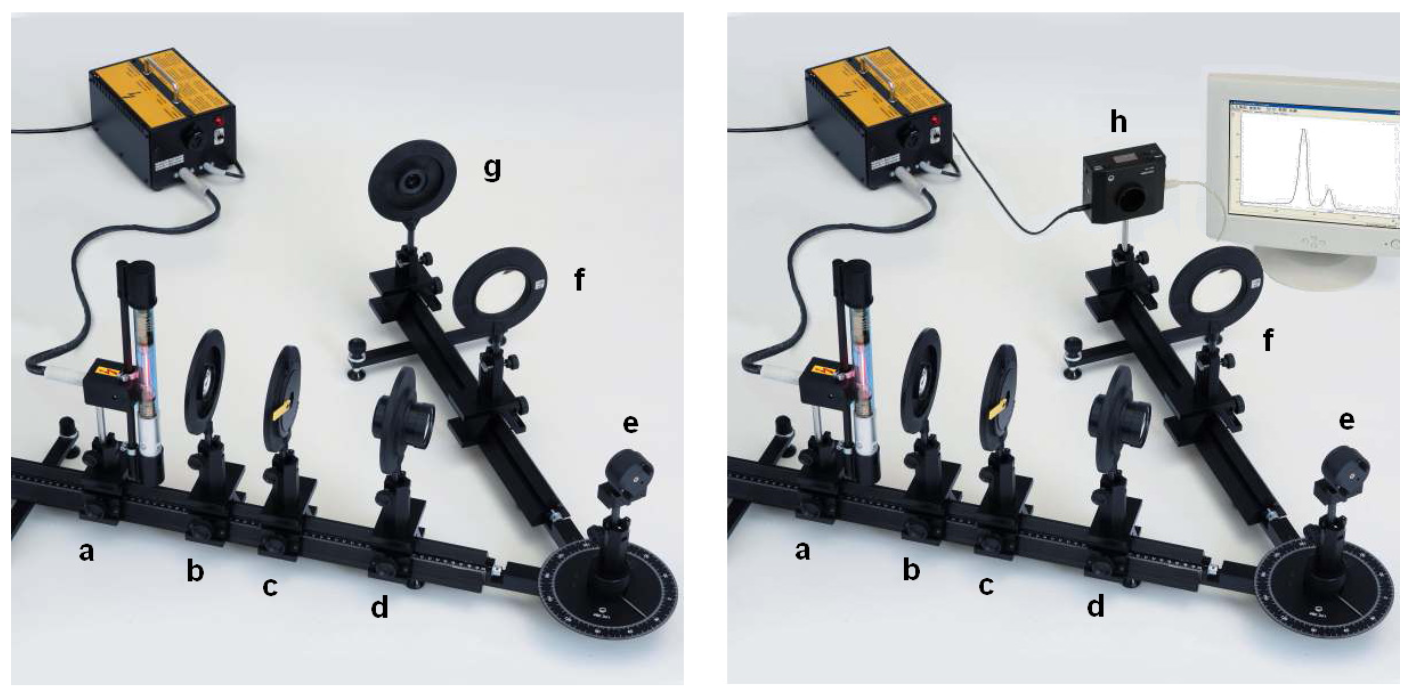
\includegraphics[width=.5\textwidth]{402_aufbau_spektrallinie.png}
        \caption{Der Aufbau zur Bestimmung der Gitterkonstanten, $R$, $h$ und der Linienverbreiterung sowie Isotopieaufspaltung.\cite{Anleitung402}} \label{fig:aufbau_spektrallinie}
\end{figure}

\subsection{Durchführung \& Auswertung:\\Gitterkonstante} \label{sec:d&a:gitterkonstante}
Der Strahlengang ist schematisch in Abb.\ (\ref{fig:strahlengang}) dargestellt.
Für jede Spektrallinie der Hg--Lampe wurde der Gitterwinkel $\omega _G$ gemessen, unter dem die Spektrallinie genau mittig auf das Okular oder die CCD trifft.
$\omega _B$ war für die gesamte Durchführung $\ang{130+-.5}$.
Die Farbe der Linie wurde mit einer Spektraltabelle \cite{Anleitung402} verglichen und so die Wellenlänge $\lambda $ bestimmt.

Die Gitterkonstante wird berechnet durch
\begin{align} 
        &&n\lambda &=g\left(\sin \alpha +\sin \beta \right)&&\\
        \Leftrightarrow &&g&=\dfrac{n\lambda }{\sin \alpha +\sin \beta },&&
\end{align} 
mit $\alpha =\omega _G$ und $\beta =\omega _B+\omega _G-\ang{180}$.
Der Fehler auf $g$ verhält sich aufgrund des Fehlers von $\omega _G$ und $\omega _B$ wie
\begin{align} 
        \Delta g &= \,\sqrt[]{\left((\partial _{\omega _G}g)\Delta \omega _G\right)^2+\left((\partial _{\omega _B}g)\Delta \omega _B\right)^2}
,\end{align} 
mit
\begin{align} 
        (\partial _{\omega _G}g)\Delta \omega _G &= \dfrac{n\lambda \Delta \omega _G\left(\cos \left(\omega _G\right)-\cos \left(\omega _B+\omega _G\right)\right)}{\left(\sin \left(\omega _G\right)-\sin \left(\omega _B+\omega _G\right)\right)^2}\\
        (\partial _{\omega _B}g)\Delta \omega _B &= \dfrac{n\lambda \Delta \omega _B\cos \left(\omega _B+\omega _G\right)}{\left(\sin \left(\omega _G\right)-\sin \left(\omega _B+\omega _G\right)\right)^2}
.\end{align} 
Trägt man $\sin \left(\omega _G\right)+\sin \left(\omega _B+\omega _B-\ang{180}\right)$ gegen die Wellenlänge $\lambda $ auf, so ergibt sich aus der Steigung der Fitgeraden die Gitterkonstante $g$.
Dies ist in Abb.\ (\ref{fig:gitterkonstante}) dargestellt.

Der Wert von $g$ ist damit
\begin{align} 
        g=\SI{4527+-47}{\text{\r{A}}^{-1}}
.\end{align} 
Der Literaturwert ist angegeben in \cite{LeyboldBalmerserieBeobachtung} und liegt bei
\begin{align} 
        g_\text{lit.}=\SI{4170}{\text{\r{A}^{-1}}}
.\end{align} 
Die Abweichung liegt bei $9\%$, also noch im akzeptablen Fehlerbereich.
Mögliche Fehler könnten durch das Ablesen des Winkels an der Winkelskala des Gitters entstanden sein, da die Einteilung nur in $\ang{1}$--Schritten angegeben ist.

Das relativ zu 1 große $\chi ^2/\text{ddof}$ ist den kleinen Fehlern geschuldet.
Die Fitgerade modelliert die Werte passend.

\begin{figure}[t]
        \centering
        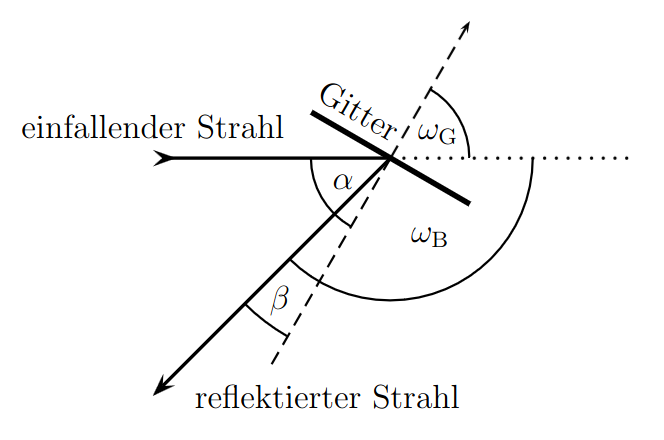
\includegraphics[width=.5\textwidth]{402_reflexion.png}
        \caption{Schematische Darstellung der Reflexion am Stufengitter.\cite{Anleitung402}} \label{fig:strahlengang}
\end{figure}
\begin{figure}[t] 
        \centering
        \resizebox{.5\textwidth}{!}{% GNUPLOT: LaTeX picture with Postscript
\begingroup
  \makeatletter
  \providecommand\color[2][]{%
    \GenericError{(gnuplot) \space\space\space\@spaces}{%
      Package color not loaded in conjunction with
      terminal option `colourtext'%
    }{See the gnuplot documentation for explanation.%
    }{Either use 'blacktext' in gnuplot or load the package
      color.sty in LaTeX.}%
    \renewcommand\color[2][]{}%
  }%
  \providecommand\includegraphics[2][]{%
    \GenericError{(gnuplot) \space\space\space\@spaces}{%
      Package graphicx or graphics not loaded%
    }{See the gnuplot documentation for explanation.%
    }{The gnuplot epslatex terminal needs graphicx.sty or graphics.sty.}%
    \renewcommand\includegraphics[2][]{}%
  }%
  \providecommand\rotatebox[2]{#2}%
  \@ifundefined{ifGPcolor}{%
    \newif\ifGPcolor
    \GPcolortrue
  }{}%
  \@ifundefined{ifGPblacktext}{%
    \newif\ifGPblacktext
    \GPblacktexttrue
  }{}%
  % define a \g@addto@macro without @ in the name:
  \let\gplgaddtomacro\g@addto@macro
  % define empty templates for all commands taking text:
  \gdef\gplbacktext{}%
  \gdef\gplfronttext{}%
  \makeatother
  \ifGPblacktext
    % no textcolor at all
    \def\colorrgb#1{}%
    \def\colorgray#1{}%
  \else
    % gray or color?
    \ifGPcolor
      \def\colorrgb#1{\color[rgb]{#1}}%
      \def\colorgray#1{\color[gray]{#1}}%
      \expandafter\def\csname LTw\endcsname{\color{white}}%
      \expandafter\def\csname LTb\endcsname{\color{black}}%
      \expandafter\def\csname LTa\endcsname{\color{black}}%
      \expandafter\def\csname LT0\endcsname{\color[rgb]{1,0,0}}%
      \expandafter\def\csname LT1\endcsname{\color[rgb]{0,1,0}}%
      \expandafter\def\csname LT2\endcsname{\color[rgb]{0,0,1}}%
      \expandafter\def\csname LT3\endcsname{\color[rgb]{1,0,1}}%
      \expandafter\def\csname LT4\endcsname{\color[rgb]{0,1,1}}%
      \expandafter\def\csname LT5\endcsname{\color[rgb]{1,1,0}}%
      \expandafter\def\csname LT6\endcsname{\color[rgb]{0,0,0}}%
      \expandafter\def\csname LT7\endcsname{\color[rgb]{1,0.3,0}}%
      \expandafter\def\csname LT8\endcsname{\color[rgb]{0.5,0.5,0.5}}%
    \else
      % gray
      \def\colorrgb#1{\color{black}}%
      \def\colorgray#1{\color[gray]{#1}}%
      \expandafter\def\csname LTw\endcsname{\color{white}}%
      \expandafter\def\csname LTb\endcsname{\color{black}}%
      \expandafter\def\csname LTa\endcsname{\color{black}}%
      \expandafter\def\csname LT0\endcsname{\color{black}}%
      \expandafter\def\csname LT1\endcsname{\color{black}}%
      \expandafter\def\csname LT2\endcsname{\color{black}}%
      \expandafter\def\csname LT3\endcsname{\color{black}}%
      \expandafter\def\csname LT4\endcsname{\color{black}}%
      \expandafter\def\csname LT5\endcsname{\color{black}}%
      \expandafter\def\csname LT6\endcsname{\color{black}}%
      \expandafter\def\csname LT7\endcsname{\color{black}}%
      \expandafter\def\csname LT8\endcsname{\color{black}}%
    \fi
  \fi
    \setlength{\unitlength}{0.0500bp}%
    \ifx\gptboxheight\undefined%
      \newlength{\gptboxheight}%
      \newlength{\gptboxwidth}%
      \newsavebox{\gptboxtext}%
    \fi%
    \setlength{\fboxrule}{0.5pt}%
    \setlength{\fboxsep}{1pt}%
    \definecolor{tbcol}{rgb}{1,1,1}%
\begin{picture}(7200.00,4320.00)%
    \gplgaddtomacro\gplbacktext{%
      \csname LTb\endcsname%%
      \put(634,619){\makebox(0,0)[r]{\strut{}$0.8$}}%
      \csname LTb\endcsname%%
      \put(634,1006){\makebox(0,0)[r]{\strut{}$0.9$}}%
      \csname LTb\endcsname%%
      \put(634,1394){\makebox(0,0)[r]{\strut{}$1$}}%
      \csname LTb\endcsname%%
      \put(634,1781){\makebox(0,0)[r]{\strut{}$1.1$}}%
      \csname LTb\endcsname%%
      \put(634,2169){\makebox(0,0)[r]{\strut{}$1.2$}}%
      \csname LTb\endcsname%%
      \put(634,2556){\makebox(0,0)[r]{\strut{}$1.3$}}%
      \csname LTb\endcsname%%
      \put(634,2944){\makebox(0,0)[r]{\strut{}$1.4$}}%
      \csname LTb\endcsname%%
      \put(634,3331){\makebox(0,0)[r]{\strut{}$1.5$}}%
      \csname LTb\endcsname%%
      \put(634,3719){\makebox(0,0)[r]{\strut{}$1.6$}}%
      \csname LTb\endcsname%%
      \put(731,425){\makebox(0,0){\strut{}$400$}}%
      \csname LTb\endcsname%%
      \put(1757,425){\makebox(0,0){\strut{}$450$}}%
      \csname LTb\endcsname%%
      \put(2783,425){\makebox(0,0){\strut{}$500$}}%
      \csname LTb\endcsname%%
      \put(3809,425){\makebox(0,0){\strut{}$550$}}%
      \csname LTb\endcsname%%
      \put(4834,425){\makebox(0,0){\strut{}$600$}}%
      \csname LTb\endcsname%%
      \put(5860,425){\makebox(0,0){\strut{}$650$}}%
      \csname LTb\endcsname%%
      \put(6886,425){\makebox(0,0){\strut{}$700$}}%
    }%
    \gplgaddtomacro\gplfronttext{%
      \csname LTb\endcsname%%
      \put(170,2169){\rotatebox{-270}{\makebox(0,0){\strut{}$[\sin{(\omega_G)}+\sin{(\omega_G+\omega_B-\SI{180}{\degree})}]/\SI{}{rad}$}}}%
      \csname LTb\endcsname%%
      \put(3809,135){\makebox(0,0){\strut{}$\lambda/\SI{}{\nano m}$}}%
      \csname LTb\endcsname%%
      \put(6123,1083){\makebox(0,0)[r]{\strut{}data}}%
      \csname LTb\endcsname%%
      \put(6123,890){\makebox(0,0)[r]{\strut{}$f(\lambda)=\frac{\lambda}{\SI{4527 +- 47}{\text{\r{A}}}}$}}%
      \csname LTb\endcsname%%
      \put(3809,4009){\makebox(0,0){\strut{}$g=\SI{4527 +- 47}{\text{\r{A}}^{-1}}$ und $\chi^2/\text{ddof}=9.920$}}%
    }%
    \gplbacktext
    \put(0,0){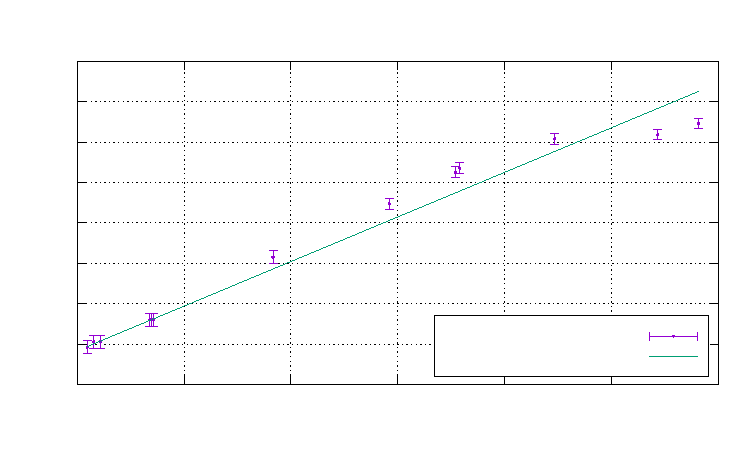
\includegraphics[width={360.00bp},height={216.00bp}]{Gitterkonstante}}%
    \gplfronttext
  \end{picture}%
\endgroup
}
        \caption{Der Gangunterschied geteilt durch die Gitterkonstante gegen die Wellenlänge aufgetragen ergibt aus der Steigung der Fitgeraden die Gitterkonstante.} \label{fig:gitterkonstante}
\end{figure}

\subsection{Durchführung \& Auswertung: Spektrallinien}
Die Hg--Lampe wurde gegen die \textsc{Balmer}--Lampe getauscht, um die Spektrallinien, genauer die Isotopieaufspaltung, der \textsc{Balmer}--Serie zu vermessen; sonst bleibt der Aufbau identisch.
Die Messung wurde mit Okular und CCD durchgeführt.
Die \textsc{Balmer}--Lampe besteht aus einem Gemisch von 10 Teilen Wasserstoff zu 1 Teil Deuterium.

Für jede Isotopieaufspaltung wurde die Distanz $d$ zwischen den Linien gemessen, um so den Wellenlängenunterschied bestimmen zu können.

\subsubsection{Okular}
Die Wellenlängen wurden analog zu Kapitel (\ref{sec:d&a:gitterkonstante}) berechnet mit 
\begin{align} 
        \lambda  &= g\left(\sin \left(\omega _G\right)+\sin \left(\omega _B+\omega _G-\ang{180}\right)\right)\\
        \Delta \lambda  &= \,\sqrt[]{\left((\partial _{\omega _G}\lambda )\Delta \omega _G\right)^2+\left( (\partial _{\omega _B}\lambda) \Delta \omega _B\right)^2},
\end{align} 
mit
\begin{align} 
        (\partial _{\omega _G}\lambda)\Delta \omega _G &= g\left(\cos \omega _G+\cos \left(\omega _B+\omega _G-\ang{180}\right)\right)\Delta \omega _G\\
        (\partial _{\omega _B}\lambda )\Delta \omega _B &= g\left(\cos \left(\omega _B+\omega _G-\ang{180}\right)\right)\Delta \omega _B
\end{align} 
Die gemessenen \textsc{Balmer}--Linien sind in Tab.\ (\ref{tab:okular}) eingetragen.
Die Messung des Winkels erfolgte durch Ablesen der Stellung des Gitters an einer Winkelskala, wenn die Linie genau im Nullpunkt der Skala des Okulars ist.
\begin{table}[h]
        \begin{tabular}{cccc}
                Farbe & $\lambda_{\text{lit.}}$ & $\lambda$ & $\omega _G$ \\
                \hline
                Rot & \SI{656}{\nano m} &\SI{741+-88}{\nano m}[13\%] & $\ang{89.5+-0.5}$ \\
                Türkis & \SI{485}{\nano m} &\SI{565+-87}{\nano m}[14\%] & $\ang{68.5+-0.5}$ \\
                Blau & \SI{433}{\nano m} &\SI{511+-86}{\nano m}[15\%] & $\ang{63.5+-0.5}$
        \end{tabular}
        \caption{$\omega _B=\ang{130}$. Messung der \textsc{Balmer}--Linien und Linienabstand mit dem Okular. Literaturwerte aus \cite{LeyboldBalmerserieBeobachtung} mit Abweichung in Klammern $[\bullet ]$.} \label{tab:okular}
\end{table}
\noindent Die Abweichung der beobachteten Wellenlängen unterscheiden sich nur geringfügig, liegen allerdings alle über $10\%$.
Diese Abweichung war nicht zu erwarten, da die Linien auf dem Okular äußert scharf waren.
Ein möglicher Grund kann die Winkelmessung gewesen sein.
Die Auflösung der Winkelskala lag lediglich bei $\ang{1}$.
Die Formel zur Wellenlängendifferenz der Isotopieauspaltung ist
\begin{align} 
        \Delta \lambda &=\dfrac{g}{n}\Delta \beta \cos \beta\\
        \Delta \left(\Delta \lambda \right) &= \,\sqrt[]{\left(\dfrac{g}{n}\cos \beta \,\Delta \left(\Delta \beta \right)\right)^2+\left(-\dfrac{g}{n}\Delta \beta \sin \beta \,\Delta \left(\beta \right)\right)^2}
,\end{align} 
mit $\Delta \left(\bullet\right)$ dem Fehler und $\Delta \bullet $ der Differenz.
Es ist $\Delta \beta =\tfrac{\Delta d}{f}$.
Daraus ergeben sich die Wellenlängendifferenzen dargestellt in Tab.\ (\ref{tab:isotopie_okular})

\begin{table}[h]
        \begin{tabular}{cccc}
                Farbe & $\Delta \lambda _\text{lit.}$ & $\Delta \lambda $ &  $d$ \\
                \hline
                Rot & $\SI{0.179}{\nano m}$& $\SI{0.274+-0.069}{\nano m}[153\%]$  & $\SI{0.2+-0.05}{mm}$ \\
                Türkis& $\SI{0.132}{\nano m}$ & $\SI{0.168+-0.084}{\nano m}[27\%]$  & $\SI{0.1+-0.05}{mm}$ \\
                Blau & $\SI{0.118}{\nano m}$& $\SI{0.863+-0.863}{\nano m}[631\%]$  & $\SI{0.05+-0.05}{mm}$ 
        \end{tabular}
        \caption{Die Wellenlängendifferenz der Isotopieaufspaltung. Literaturwerte aus \cite{LeyboldBalmerserieBeobachtung} mit Abweichung in Klammern $[\bullet ]$.} \label{tab:isotopie_okular}
\end{table}
Der Fehler der blauen Aufspaltung ist besonders groß, weil der Linienabstand eine Größe von einem Skalenteil hatte.
Die sehr großen Abweichungen von Rot und vor Allem Türkis waren nicht zu erwarten.
Die rote und türkisfarbene Linie konnte sehr präzise aufgelöst werden, sodass Fehler nicht durch Unschärfe kommen konnten.
Die Möglichkeiten einer solch geringen Aufspaltung waren durch das Okular und die Skalenteile von $\SI{0.01}{mm}$ begrenzt, was ein Grund für diese Abweichungen sein könnte.
Die Abweichung der blauen Linie ist zu groß, als dass die Skala im Okular hier eine Rolle spielen könnte.
Da die blaue Linie eine geringe Intensität hatte, ist die Möglichkeit einer präzisen Messung schwierig gewesen, was zu diesem großen Fehler und auch zu der großen Abweichung geführt hat.

\subsubsection{CCD}
Für die Messung mit der CCD wurde das Okular durch eine CCD--Kamera ausgetauscht.
Die Datenentnahme erfolgte über einen PC.
Die Messung sind in Abb.\ (\ref{fig:ccdrot}) bis Abb.\ (\ref{fig:ccdvioletstark}) zu sehen.

Der Fit der Daten wurde mit zwei \textsc{Gauss}--Kurven der Form
\begin{align} 
        f\left(x\right)=b_1\text{exp}\left(-\dfrac{\left(x-c_1\right)^2}{a_1}\right)+b_2\text{exp}\left(-\dfrac{\left(x-c_2\right)^2}{a_2}\right)+g
\end{align} 
durchgeführt.
Die Parameter, die sich aus dem Fit ergeben haben sind in einer Tabelle unter jedem Plot im Appendix zu finden.
Die Wellenlängen berechnen sich analog zum Okular.
Die Nulllage ist die Nulllinie der CCD, die auf dem PC zu beobachten war.
Es ergaben sich die Wellenlängen aus Tab.\ (\ref{tab:isotopie_ccd}).

\begin{table}[h]
        \begin{tabular}{cccc}
                Farbe & $\lambda_{\text{lit.}}$ & $\lambda$ & $\omega _G$ \\
                \hline
                Rot & \SI{656}{\nano m} &\SI{696+-190}{\nano m}[6\%] & $\ang{83.0+-0.5}$ \\
                Türkis & \SI{485}{\nano m} &\SI{499+-221}{\nano m}[3\%] & $\ang{62.5+-0.5}$ \\
                Violet Schwach & $\SI{434}{\nano m}$ &\SI{441+-225}{\nano m}[2\%] & $\ang{57.5+-0.5}$ \\
        Violet Stark & $\SI{410}{\nano m}$ &\SI{435+-225}{\nano m}[6\%] & $\ang{57.0+-0.5}$ 
        \end{tabular}
        \caption{$\omega _B=\ang{130}$. Wellenlängen der \textsc{Balmer}--Serie berechnet mit Hilfe der CCD. Literaturwerte aus \cite{LeyboldBalmerserieBeobachtung} mit Abweichung in Klammern $[\bullet ]$.} \label{tab:isotopie_ccd}
\end{table}
Zu erkennen ist, dass die Abweichung aller Wellenlängen unter $10\%$ liegt.
Dieses Ergebnis ist im Vergleich zum Okular viel besser, was daran liegt, dass mit der CCD eine viel größere Auflösung für die Nulllage erreicht werden kann.

Die Isotopieaufspaltung berechnet sich aus dem Abstand der Maxima der \textsc{Gauss}--Kurven, der Winkeldifferenz.

\begin{table}[h]
        \begin{tabular}{ccc}
                Farbe & $\Delta \lambda_{\text{lit.}}$ & $\Delta \lambda$\\
                \hline
                Rot & $\SI{0.179}{\nano m}$ & \SI{0.215+-0.070}{\nano m}[20\%]\\
                Türkis & $\SI{0.132}{\nano m}$ & \SI{0.283+-0.319}{\nano m}[114\%]\\
                Violet schwach & $\SI{0.118}{\nano m}$ & \SI{0.271+-0.291}{\nano m}[130\%]\\
                Violet stark & $\SI{0.112}{\nano m}$ & \SI{0.286+-0.273}{\nano m}[155\%]
        \end{tabular}
        \caption{Isotopieaufspaltung berechnet mit Hilfe der CCD. Literaturwerte aus \cite{LeyboldBalmerserieBeobachtung} mit Abweichung in Klammern $[\bullet ]$.} \label{tab:isotopie_ccd}
\end{table}
Die Fehler sind, für die Präzision mit der die Wellenlängen der \textsc{Balmer}--Serie gemessen worden sind, unerwartet.
Die Fehler steigen mit kleiner werdender Wellenlänge, da für diese Wellenlängen die Intensitäten geringer und die Linien breiter wurden, wodurch die Bestimmung des Maximums erschwert worden ist.
Eine Steigerung war also zu erwarten, allerdings nicht in dieser Größenordnung.
Der Fehler für die rote Linie ist im Vergleich noch akzeptabel.

\subsubsection{Durchführung \& Auswertung: \textsc{Rydberg}--Konstante}
Die \textsc{Rydberg}--Konstante bestimmt sich aus der Energiedifferenz der \textsc{Balmer}--$\alpha $, --$\beta $, --$\gamma $ und --$\delta $ Übergänge.
Die gemessene Wellenlänge ist mit der Energie über $E=h\tfrac{c}{\lambda }$ verknüpft.
Man berechnet für jede Wellenlänge die \textsc{Rydberg}--Konstante mit
\begin{align} 
        R_\infty=\dfrac{\tfrac{c}{\lambda }}{\tfrac{1}{n_<^2}-\tfrac{1}{n_>^2}}=\dfrac{\tfrac{c}{\lambda }n_<^2n_>^2}{n_>^2-n_<^2}
.\end{align} 
Das \textsc{Plack}'sche Wirkungsquantum wird dann über die \textsc{Rydberg}--Konstante bestimmt, mit
\begin{align} 
        h=\,\sqrt[3]{\dfrac{m_e e^4}{8\varepsilon _0^2R_\infty c}}
.\end{align} 
Die spezifische \textsc{Rydberg}--Konstante für Wasserstoff liegt dann mit der reduzierten Masse $\mu =\tfrac{m_em_K}{m_e+m_K}\approx m_e$, da $m_e\ll m_K$, bei
\begin{align} 
        R_\infty=\dfrac{R_\text{H}}{\mu }
.\end{align} 
Es ergeben sich folgende Größen
\begin{align} 
        R_\infty&=\SI{0.923+-0.047}{10^{-7}/m}[16\%]\\
        R_{H}&=\SI{0.923+-0.047}{10^{-7}/m}\\
        h_R&=\SI{7.01+-0.35}{10^{-34}J/Hz}[6\%]\approx \SI{4.38e-15}{J/Hz}
\end{align} 
In Klammern ist die Abweichung vom CODATA\cite{CODATA} Wert
\begin{align} 
        R_{\infty,\text{CODATA}}&\approx \SI{1.0973e-7}{1/m}\\
        h_\text{CODATA}&\approx \SI{6.626}{J/Hz}
.\end{align} 
Der Wert der \textsc{Rydberg}--Konstante ist über den $10\%$ Toleranz.
Grund hierfür sind die großen Abweichungen von der Literatur der gemessenen Wellenlängen.
Obwohl die Abweichung nicht unerheblich ist, liegt sie bei dem \textsc{Planck}'schen Wirkungsquantum nur bei $6\%$.
Vergleicht man diesen Wert mit dem aus Kapitel (\ref{sec:photoeffekt}) zum Photoeffekt, so weicht dieser Wert um nur 2\% ab.
Dies spricht für sehr konsistente Messergebnisse innerhalb der Fehlergrenzen.

%Warum ist der Wert so schlecht, wenn R_H doch so gut ist????? jonas
%ich glaub die sind gar nicht so schlecht 



\section{Fazit}

%{{{ appendix & bibliography
\clearpage
\section{Appendix}
\begin{figure}[h]
        \centering
        \resizebox{.5\textwidth}{!}{% GNUPLOT: LaTeX picture with Postscript
\begingroup
  \makeatletter
  \providecommand\color[2][]{%
    \GenericError{(gnuplot) \space\space\space\@spaces}{%
      Package color not loaded in conjunction with
      terminal option `colourtext'%
    }{See the gnuplot documentation for explanation.%
    }{Either use 'blacktext' in gnuplot or load the package
      color.sty in LaTeX.}%
    \renewcommand\color[2][]{}%
  }%
  \providecommand\includegraphics[2][]{%
    \GenericError{(gnuplot) \space\space\space\@spaces}{%
      Package graphicx or graphics not loaded%
    }{See the gnuplot documentation for explanation.%
    }{The gnuplot epslatex terminal needs graphicx.sty or graphics.sty.}%
    \renewcommand\includegraphics[2][]{}%
  }%
  \providecommand\rotatebox[2]{#2}%
  \@ifundefined{ifGPcolor}{%
    \newif\ifGPcolor
    \GPcolortrue
  }{}%
  \@ifundefined{ifGPblacktext}{%
    \newif\ifGPblacktext
    \GPblacktexttrue
  }{}%
  % define a \g@addto@macro without @ in the name:
  \let\gplgaddtomacro\g@addto@macro
  % define empty templates for all commands taking text:
  \gdef\gplbacktext{}%
  \gdef\gplfronttext{}%
  \makeatother
  \ifGPblacktext
    % no textcolor at all
    \def\colorrgb#1{}%
    \def\colorgray#1{}%
  \else
    % gray or color?
    \ifGPcolor
      \def\colorrgb#1{\color[rgb]{#1}}%
      \def\colorgray#1{\color[gray]{#1}}%
      \expandafter\def\csname LTw\endcsname{\color{white}}%
      \expandafter\def\csname LTb\endcsname{\color{black}}%
      \expandafter\def\csname LTa\endcsname{\color{black}}%
      \expandafter\def\csname LT0\endcsname{\color[rgb]{1,0,0}}%
      \expandafter\def\csname LT1\endcsname{\color[rgb]{0,1,0}}%
      \expandafter\def\csname LT2\endcsname{\color[rgb]{0,0,1}}%
      \expandafter\def\csname LT3\endcsname{\color[rgb]{1,0,1}}%
      \expandafter\def\csname LT4\endcsname{\color[rgb]{0,1,1}}%
      \expandafter\def\csname LT5\endcsname{\color[rgb]{1,1,0}}%
      \expandafter\def\csname LT6\endcsname{\color[rgb]{0,0,0}}%
      \expandafter\def\csname LT7\endcsname{\color[rgb]{1,0.3,0}}%
      \expandafter\def\csname LT8\endcsname{\color[rgb]{0.5,0.5,0.5}}%
    \else
      % gray
      \def\colorrgb#1{\color{black}}%
      \def\colorgray#1{\color[gray]{#1}}%
      \expandafter\def\csname LTw\endcsname{\color{white}}%
      \expandafter\def\csname LTb\endcsname{\color{black}}%
      \expandafter\def\csname LTa\endcsname{\color{black}}%
      \expandafter\def\csname LT0\endcsname{\color{black}}%
      \expandafter\def\csname LT1\endcsname{\color{black}}%
      \expandafter\def\csname LT2\endcsname{\color{black}}%
      \expandafter\def\csname LT3\endcsname{\color{black}}%
      \expandafter\def\csname LT4\endcsname{\color{black}}%
      \expandafter\def\csname LT5\endcsname{\color{black}}%
      \expandafter\def\csname LT6\endcsname{\color{black}}%
      \expandafter\def\csname LT7\endcsname{\color{black}}%
      \expandafter\def\csname LT8\endcsname{\color{black}}%
    \fi
  \fi
    \setlength{\unitlength}{0.0500bp}%
    \ifx\gptboxheight\undefined%
      \newlength{\gptboxheight}%
      \newlength{\gptboxwidth}%
      \newsavebox{\gptboxtext}%
    \fi%
    \setlength{\fboxrule}{0.5pt}%
    \setlength{\fboxsep}{1pt}%
    \definecolor{tbcol}{rgb}{1,1,1}%
\begin{picture}(7200.00,4320.00)%
    \gplgaddtomacro\gplbacktext{%
      \csname LTb\endcsname%%
      \put(536,619){\makebox(0,0)[r]{\strut{}$-2$}}%
      \csname LTb\endcsname%%
      \put(536,1135){\makebox(0,0)[r]{\strut{}$0$}}%
      \csname LTb\endcsname%%
      \put(536,1652){\makebox(0,0)[r]{\strut{}$2$}}%
      \csname LTb\endcsname%%
      \put(536,2169){\makebox(0,0)[r]{\strut{}$4$}}%
      \csname LTb\endcsname%%
      \put(536,2686){\makebox(0,0)[r]{\strut{}$6$}}%
      \csname LTb\endcsname%%
      \put(536,3202){\makebox(0,0)[r]{\strut{}$8$}}%
      \csname LTb\endcsname%%
      \put(536,3719){\makebox(0,0)[r]{\strut{}$10$}}%
      \csname LTb\endcsname%%
      \put(634,425){\makebox(0,0){\strut{}$-2.5$}}%
      \csname LTb\endcsname%%
      \put(1836,425){\makebox(0,0){\strut{}$-2$}}%
      \csname LTb\endcsname%%
      \put(3038,425){\makebox(0,0){\strut{}$-1.5$}}%
      \csname LTb\endcsname%%
      \put(4241,425){\makebox(0,0){\strut{}$-1$}}%
      \csname LTb\endcsname%%
      \put(5443,425){\makebox(0,0){\strut{}$-0.5$}}%
      \csname LTb\endcsname%%
      \put(6645,425){\makebox(0,0){\strut{}$0$}}%
    }%
    \gplgaddtomacro\gplfronttext{%
      \csname LTb\endcsname%%
      \put(4550,3448){\makebox(0,0)[r]{\strut{}quadratische Datenpunkte}}%
      \csname LTb\endcsname%%
      \put(4550,3255){\makebox(0,0)[r]{\strut{}nicht quadratische Datenpunkte}}%
      \csname LTb\endcsname%%
      \put(4550,3061){\makebox(0,0)[r]{\strut{}$f(x)=\SI{7.199 +- 0.054}{}\cdot U_G + \SI{8.499 +- 0.020}{\milli V}$}}%
      \csname LTb\endcsname%%
      \put(170,2169){\rotatebox{-270.00}{\makebox(0,0){\strut{}$\sqrt{I-I_0}$/mV}}}%
      \csname LTb\endcsname%%
      \put(3760,135){\makebox(0,0){\strut{}$U_G$/V}}%
      \csname LTb\endcsname%%
      \put(3760,4009){\makebox(0,0){\strut{}$\lambda=\SI{305}{\nano m}$: $U_0=\SI{-1.1806 +- 0.0093}{V}$ und $\chi^2/\text{ddof}=\SI{0.040}{}$}}%
    }%
    \gplbacktext
    \put(0,0){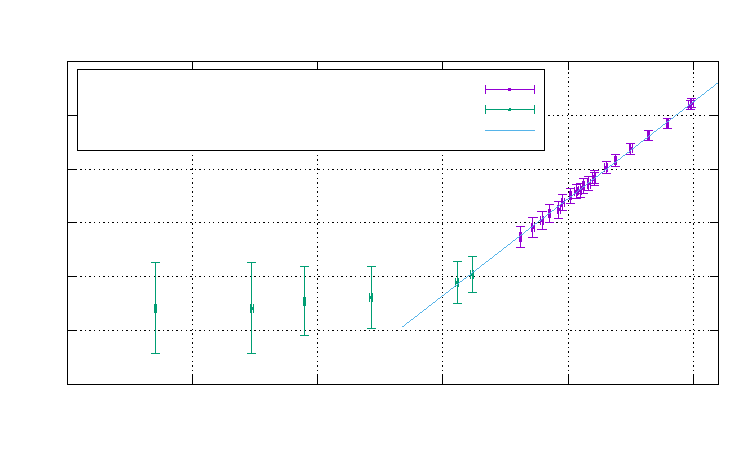
\includegraphics[width={360.00bp},height={216.00bp}]{305nm}}%
    \gplfronttext
  \end{picture}%
\endgroup
}
        \caption{Photostrom abzüglich des Anodenstroms gegen Gegenspannung für $\lambda =\SI{305}{n m}$. Fit nur an Messdaten quadratisch ab $U_0$ und in quadratischer Abhängigkeit.} \label{fig:photo_auswertung_305}
\end{figure}
\begin{figure}[h]
        \centering
        \resizebox{.5\textwidth}{!}{% GNUPLOT: LaTeX picture with Postscript
\begingroup
  \makeatletter
  \providecommand\color[2][]{%
    \GenericError{(gnuplot) \space\space\space\@spaces}{%
      Package color not loaded in conjunction with
      terminal option `colourtext'%
    }{See the gnuplot documentation for explanation.%
    }{Either use 'blacktext' in gnuplot or load the package
      color.sty in LaTeX.}%
    \renewcommand\color[2][]{}%
  }%
  \providecommand\includegraphics[2][]{%
    \GenericError{(gnuplot) \space\space\space\@spaces}{%
      Package graphicx or graphics not loaded%
    }{See the gnuplot documentation for explanation.%
    }{The gnuplot epslatex terminal needs graphicx.sty or graphics.sty.}%
    \renewcommand\includegraphics[2][]{}%
  }%
  \providecommand\rotatebox[2]{#2}%
  \@ifundefined{ifGPcolor}{%
    \newif\ifGPcolor
    \GPcolortrue
  }{}%
  \@ifundefined{ifGPblacktext}{%
    \newif\ifGPblacktext
    \GPblacktexttrue
  }{}%
  % define a \g@addto@macro without @ in the name:
  \let\gplgaddtomacro\g@addto@macro
  % define empty templates for all commands taking text:
  \gdef\gplbacktext{}%
  \gdef\gplfronttext{}%
  \makeatother
  \ifGPblacktext
    % no textcolor at all
    \def\colorrgb#1{}%
    \def\colorgray#1{}%
  \else
    % gray or color?
    \ifGPcolor
      \def\colorrgb#1{\color[rgb]{#1}}%
      \def\colorgray#1{\color[gray]{#1}}%
      \expandafter\def\csname LTw\endcsname{\color{white}}%
      \expandafter\def\csname LTb\endcsname{\color{black}}%
      \expandafter\def\csname LTa\endcsname{\color{black}}%
      \expandafter\def\csname LT0\endcsname{\color[rgb]{1,0,0}}%
      \expandafter\def\csname LT1\endcsname{\color[rgb]{0,1,0}}%
      \expandafter\def\csname LT2\endcsname{\color[rgb]{0,0,1}}%
      \expandafter\def\csname LT3\endcsname{\color[rgb]{1,0,1}}%
      \expandafter\def\csname LT4\endcsname{\color[rgb]{0,1,1}}%
      \expandafter\def\csname LT5\endcsname{\color[rgb]{1,1,0}}%
      \expandafter\def\csname LT6\endcsname{\color[rgb]{0,0,0}}%
      \expandafter\def\csname LT7\endcsname{\color[rgb]{1,0.3,0}}%
      \expandafter\def\csname LT8\endcsname{\color[rgb]{0.5,0.5,0.5}}%
    \else
      % gray
      \def\colorrgb#1{\color{black}}%
      \def\colorgray#1{\color[gray]{#1}}%
      \expandafter\def\csname LTw\endcsname{\color{white}}%
      \expandafter\def\csname LTb\endcsname{\color{black}}%
      \expandafter\def\csname LTa\endcsname{\color{black}}%
      \expandafter\def\csname LT0\endcsname{\color{black}}%
      \expandafter\def\csname LT1\endcsname{\color{black}}%
      \expandafter\def\csname LT2\endcsname{\color{black}}%
      \expandafter\def\csname LT3\endcsname{\color{black}}%
      \expandafter\def\csname LT4\endcsname{\color{black}}%
      \expandafter\def\csname LT5\endcsname{\color{black}}%
      \expandafter\def\csname LT6\endcsname{\color{black}}%
      \expandafter\def\csname LT7\endcsname{\color{black}}%
      \expandafter\def\csname LT8\endcsname{\color{black}}%
    \fi
  \fi
    \setlength{\unitlength}{0.0500bp}%
    \ifx\gptboxheight\undefined%
      \newlength{\gptboxheight}%
      \newlength{\gptboxwidth}%
      \newsavebox{\gptboxtext}%
    \fi%
    \setlength{\fboxrule}{0.5pt}%
    \setlength{\fboxsep}{1pt}%
    \definecolor{tbcol}{rgb}{1,1,1}%
\begin{picture}(7200.00,4320.00)%
    \gplgaddtomacro\gplbacktext{%
      \csname LTb\endcsname%%
      \put(536,619){\makebox(0,0)[r]{\strut{}$-4$}}%
      \csname LTb\endcsname%%
      \put(536,963){\makebox(0,0)[r]{\strut{}$-2$}}%
      \csname LTb\endcsname%%
      \put(536,1308){\makebox(0,0)[r]{\strut{}$0$}}%
      \csname LTb\endcsname%%
      \put(536,1652){\makebox(0,0)[r]{\strut{}$2$}}%
      \csname LTb\endcsname%%
      \put(536,1997){\makebox(0,0)[r]{\strut{}$4$}}%
      \csname LTb\endcsname%%
      \put(536,2341){\makebox(0,0)[r]{\strut{}$6$}}%
      \csname LTb\endcsname%%
      \put(536,2686){\makebox(0,0)[r]{\strut{}$8$}}%
      \csname LTb\endcsname%%
      \put(536,3030){\makebox(0,0)[r]{\strut{}$10$}}%
      \csname LTb\endcsname%%
      \put(536,3374){\makebox(0,0)[r]{\strut{}$12$}}%
      \csname LTb\endcsname%%
      \put(536,3719){\makebox(0,0)[r]{\strut{}$14$}}%
      \csname LTb\endcsname%%
      \put(634,425){\makebox(0,0){\strut{}$-2.5$}}%
      \csname LTb\endcsname%%
      \put(1836,425){\makebox(0,0){\strut{}$-2$}}%
      \csname LTb\endcsname%%
      \put(3038,425){\makebox(0,0){\strut{}$-1.5$}}%
      \csname LTb\endcsname%%
      \put(4241,425){\makebox(0,0){\strut{}$-1$}}%
      \csname LTb\endcsname%%
      \put(5443,425){\makebox(0,0){\strut{}$-0.5$}}%
      \csname LTb\endcsname%%
      \put(6645,425){\makebox(0,0){\strut{}$0$}}%
    }%
    \gplgaddtomacro\gplfronttext{%
      \csname LTb\endcsname%%
      \put(170,2169){\rotatebox{-270}{\makebox(0,0){\strut{}$\sqrt{I-I_0}$/mV}}}%
      \csname LTb\endcsname%%
      \put(3760,135){\makebox(0,0){\strut{}$U_G$/V}}%
      \csname LTb\endcsname%%
      \put(4745,3545){\makebox(0,0)[r]{\strut{}quadratische Datenpunkte}}%
      \csname LTb\endcsname%%
      \put(4745,3351){\makebox(0,0)[r]{\strut{}nicht quadratische Datenpunkte}}%
      \csname LTb\endcsname%%
      \put(4745,3158){\makebox(0,0)[r]{\strut{}$f(U_G)=\SI{7.649 +- 0.083}{}\cdot U_G + \SI{11.543 +- 0.040}{\milli V}$}}%
      \csname LTb\endcsname%%
      \put(3760,4009){\makebox(0,0){\strut{}$\lambda=\SI{365}{\nano m}$: $U_0=\SI{-1.509 +- 0.017}{V}$ und $\chi^2/\text{ddof}=\SI{0.389}{}$}}%
    }%
    \gplbacktext
    \put(0,0){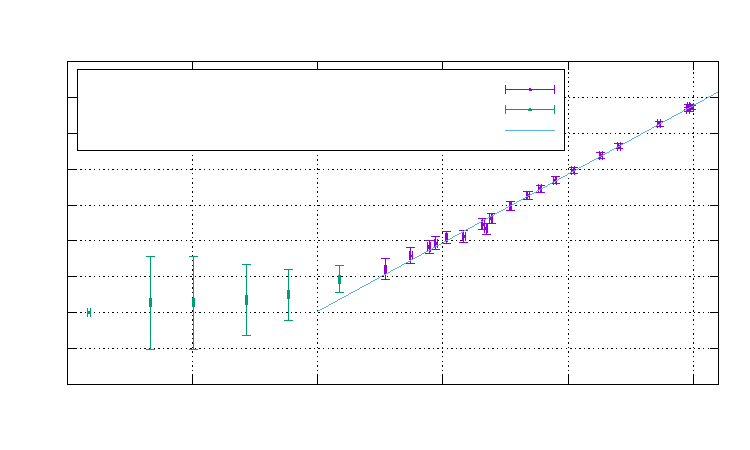
\includegraphics[width={360.00bp},height={216.00bp}]{365nm}}%
    \gplfronttext
  \end{picture}%
\endgroup
}
        \caption{Photostrom abzüglich des Anodenstroms gegen Gegenspannung für $\lambda =\SI{365}{n m}$. Fit nur an Messdaten quadratisch ab $U_0$ und in quadratischer Abhängigkeit.}
\end{figure}
\begin{figure}[h]
        \centering
        \resizebox{.5\textwidth}{!}{% GNUPLOT: LaTeX picture with Postscript
\begingroup
  \makeatletter
  \providecommand\color[2][]{%
    \GenericError{(gnuplot) \space\space\space\@spaces}{%
      Package color not loaded in conjunction with
      terminal option `colourtext'%
    }{See the gnuplot documentation for explanation.%
    }{Either use 'blacktext' in gnuplot or load the package
      color.sty in LaTeX.}%
    \renewcommand\color[2][]{}%
  }%
  \providecommand\includegraphics[2][]{%
    \GenericError{(gnuplot) \space\space\space\@spaces}{%
      Package graphicx or graphics not loaded%
    }{See the gnuplot documentation for explanation.%
    }{The gnuplot epslatex terminal needs graphicx.sty or graphics.sty.}%
    \renewcommand\includegraphics[2][]{}%
  }%
  \providecommand\rotatebox[2]{#2}%
  \@ifundefined{ifGPcolor}{%
    \newif\ifGPcolor
    \GPcolortrue
  }{}%
  \@ifundefined{ifGPblacktext}{%
    \newif\ifGPblacktext
    \GPblacktexttrue
  }{}%
  % define a \g@addto@macro without @ in the name:
  \let\gplgaddtomacro\g@addto@macro
  % define empty templates for all commands taking text:
  \gdef\gplbacktext{}%
  \gdef\gplfronttext{}%
  \makeatother
  \ifGPblacktext
    % no textcolor at all
    \def\colorrgb#1{}%
    \def\colorgray#1{}%
  \else
    % gray or color?
    \ifGPcolor
      \def\colorrgb#1{\color[rgb]{#1}}%
      \def\colorgray#1{\color[gray]{#1}}%
      \expandafter\def\csname LTw\endcsname{\color{white}}%
      \expandafter\def\csname LTb\endcsname{\color{black}}%
      \expandafter\def\csname LTa\endcsname{\color{black}}%
      \expandafter\def\csname LT0\endcsname{\color[rgb]{1,0,0}}%
      \expandafter\def\csname LT1\endcsname{\color[rgb]{0,1,0}}%
      \expandafter\def\csname LT2\endcsname{\color[rgb]{0,0,1}}%
      \expandafter\def\csname LT3\endcsname{\color[rgb]{1,0,1}}%
      \expandafter\def\csname LT4\endcsname{\color[rgb]{0,1,1}}%
      \expandafter\def\csname LT5\endcsname{\color[rgb]{1,1,0}}%
      \expandafter\def\csname LT6\endcsname{\color[rgb]{0,0,0}}%
      \expandafter\def\csname LT7\endcsname{\color[rgb]{1,0.3,0}}%
      \expandafter\def\csname LT8\endcsname{\color[rgb]{0.5,0.5,0.5}}%
    \else
      % gray
      \def\colorrgb#1{\color{black}}%
      \def\colorgray#1{\color[gray]{#1}}%
      \expandafter\def\csname LTw\endcsname{\color{white}}%
      \expandafter\def\csname LTb\endcsname{\color{black}}%
      \expandafter\def\csname LTa\endcsname{\color{black}}%
      \expandafter\def\csname LT0\endcsname{\color{black}}%
      \expandafter\def\csname LT1\endcsname{\color{black}}%
      \expandafter\def\csname LT2\endcsname{\color{black}}%
      \expandafter\def\csname LT3\endcsname{\color{black}}%
      \expandafter\def\csname LT4\endcsname{\color{black}}%
      \expandafter\def\csname LT5\endcsname{\color{black}}%
      \expandafter\def\csname LT6\endcsname{\color{black}}%
      \expandafter\def\csname LT7\endcsname{\color{black}}%
      \expandafter\def\csname LT8\endcsname{\color{black}}%
    \fi
  \fi
    \setlength{\unitlength}{0.0500bp}%
    \ifx\gptboxheight\undefined%
      \newlength{\gptboxheight}%
      \newlength{\gptboxwidth}%
      \newsavebox{\gptboxtext}%
    \fi%
    \setlength{\fboxrule}{0.5pt}%
    \setlength{\fboxsep}{1pt}%
    \definecolor{tbcol}{rgb}{1,1,1}%
\begin{picture}(7200.00,4320.00)%
    \gplgaddtomacro\gplbacktext{%
      \csname LTb\endcsname%%
      \put(536,766){\makebox(0,0)[r]{\strut{}$0$}}%
      \csname LTb\endcsname%%
      \put(536,1357){\makebox(0,0)[r]{\strut{}$2$}}%
      \csname LTb\endcsname%%
      \put(536,1947){\makebox(0,0)[r]{\strut{}$4$}}%
      \csname LTb\endcsname%%
      \put(536,2538){\makebox(0,0)[r]{\strut{}$6$}}%
      \csname LTb\endcsname%%
      \put(536,3128){\makebox(0,0)[r]{\strut{}$8$}}%
      \csname LTb\endcsname%%
      \put(536,3719){\makebox(0,0)[r]{\strut{}$10$}}%
      \csname LTb\endcsname%%
      \put(634,425){\makebox(0,0){\strut{}$-2.5$}}%
      \csname LTb\endcsname%%
      \put(1836,425){\makebox(0,0){\strut{}$-2$}}%
      \csname LTb\endcsname%%
      \put(3038,425){\makebox(0,0){\strut{}$-1.5$}}%
      \csname LTb\endcsname%%
      \put(4241,425){\makebox(0,0){\strut{}$-1$}}%
      \csname LTb\endcsname%%
      \put(5443,425){\makebox(0,0){\strut{}$-0.5$}}%
      \csname LTb\endcsname%%
      \put(6645,425){\makebox(0,0){\strut{}$0$}}%
    }%
    \gplgaddtomacro\gplfronttext{%
      \csname LTb\endcsname%%
      \put(4256,3448){\makebox(0,0)[r]{\strut{}quadratische Datenpunkte}}%
      \csname LTb\endcsname%%
      \put(4256,3255){\makebox(0,0)[r]{\strut{}nicht quadratische Datenpunkte}}%
      \csname LTb\endcsname%%
      \put(4256,3061){\makebox(0,0)[r]{\strut{}$f(U_G)=\SI{9.02 +- 0.10}{}\cdot U_G + \SI{8.575 +- 0.027}{\milli V}$}}%
      \csname LTb\endcsname%%
      \put(170,2169){\rotatebox{-270.00}{\makebox(0,0){\strut{}$\sqrt{I-I_0}$/mV}}}%
      \csname LTb\endcsname%%
      \put(3760,135){\makebox(0,0){\strut{}$U_G$/V}}%
      \csname LTb\endcsname%%
      \put(3760,4009){\makebox(0,0){\strut{}$\lambda=\SI{436}{\nano m}$: $U_0=\SI{-0.951 +- 0.000}{V}$ und $\chi^2/\text{ddof}=\SI{0.103}{}$}}%
    }%
    \gplbacktext
    \put(0,0){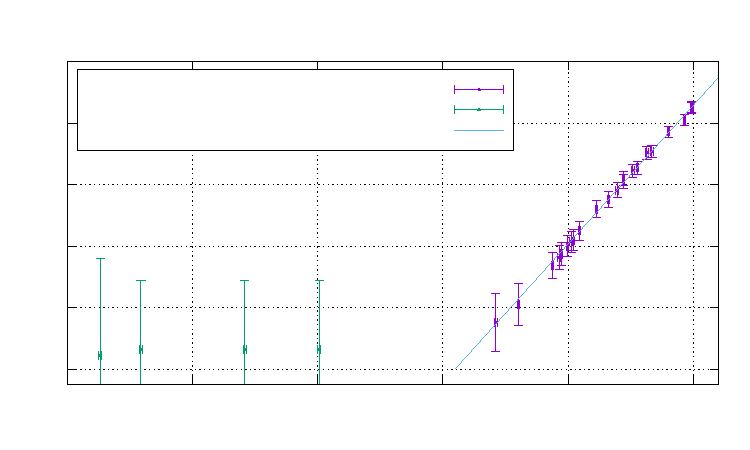
\includegraphics[width={360.00bp},height={216.00bp}]{436nm}}%
    \gplfronttext
  \end{picture}%
\endgroup
}
        \caption{Photostrom abzüglich des Anodenstroms gegen Gegenspannung für $\lambda =\SI{436}{n m}$. Fit nur an Messdaten quadratisch ab $U_0$ und in quadratischer Abhängigkeit.}
\end{figure}
\begin{figure}[h]
        \centering
        \resizebox{.5\textwidth}{!}{% GNUPLOT: LaTeX picture with Postscript
\begingroup
  \makeatletter
  \providecommand\color[2][]{%
    \GenericError{(gnuplot) \space\space\space\@spaces}{%
      Package color not loaded in conjunction with
      terminal option `colourtext'%
    }{See the gnuplot documentation for explanation.%
    }{Either use 'blacktext' in gnuplot or load the package
      color.sty in LaTeX.}%
    \renewcommand\color[2][]{}%
  }%
  \providecommand\includegraphics[2][]{%
    \GenericError{(gnuplot) \space\space\space\@spaces}{%
      Package graphicx or graphics not loaded%
    }{See the gnuplot documentation for explanation.%
    }{The gnuplot epslatex terminal needs graphicx.sty or graphics.sty.}%
    \renewcommand\includegraphics[2][]{}%
  }%
  \providecommand\rotatebox[2]{#2}%
  \@ifundefined{ifGPcolor}{%
    \newif\ifGPcolor
    \GPcolortrue
  }{}%
  \@ifundefined{ifGPblacktext}{%
    \newif\ifGPblacktext
    \GPblacktexttrue
  }{}%
  % define a \g@addto@macro without @ in the name:
  \let\gplgaddtomacro\g@addto@macro
  % define empty templates for all commands taking text:
  \gdef\gplbacktext{}%
  \gdef\gplfronttext{}%
  \makeatother
  \ifGPblacktext
    % no textcolor at all
    \def\colorrgb#1{}%
    \def\colorgray#1{}%
  \else
    % gray or color?
    \ifGPcolor
      \def\colorrgb#1{\color[rgb]{#1}}%
      \def\colorgray#1{\color[gray]{#1}}%
      \expandafter\def\csname LTw\endcsname{\color{white}}%
      \expandafter\def\csname LTb\endcsname{\color{black}}%
      \expandafter\def\csname LTa\endcsname{\color{black}}%
      \expandafter\def\csname LT0\endcsname{\color[rgb]{1,0,0}}%
      \expandafter\def\csname LT1\endcsname{\color[rgb]{0,1,0}}%
      \expandafter\def\csname LT2\endcsname{\color[rgb]{0,0,1}}%
      \expandafter\def\csname LT3\endcsname{\color[rgb]{1,0,1}}%
      \expandafter\def\csname LT4\endcsname{\color[rgb]{0,1,1}}%
      \expandafter\def\csname LT5\endcsname{\color[rgb]{1,1,0}}%
      \expandafter\def\csname LT6\endcsname{\color[rgb]{0,0,0}}%
      \expandafter\def\csname LT7\endcsname{\color[rgb]{1,0.3,0}}%
      \expandafter\def\csname LT8\endcsname{\color[rgb]{0.5,0.5,0.5}}%
    \else
      % gray
      \def\colorrgb#1{\color{black}}%
      \def\colorgray#1{\color[gray]{#1}}%
      \expandafter\def\csname LTw\endcsname{\color{white}}%
      \expandafter\def\csname LTb\endcsname{\color{black}}%
      \expandafter\def\csname LTa\endcsname{\color{black}}%
      \expandafter\def\csname LT0\endcsname{\color{black}}%
      \expandafter\def\csname LT1\endcsname{\color{black}}%
      \expandafter\def\csname LT2\endcsname{\color{black}}%
      \expandafter\def\csname LT3\endcsname{\color{black}}%
      \expandafter\def\csname LT4\endcsname{\color{black}}%
      \expandafter\def\csname LT5\endcsname{\color{black}}%
      \expandafter\def\csname LT6\endcsname{\color{black}}%
      \expandafter\def\csname LT7\endcsname{\color{black}}%
      \expandafter\def\csname LT8\endcsname{\color{black}}%
    \fi
  \fi
    \setlength{\unitlength}{0.0500bp}%
    \ifx\gptboxheight\undefined%
      \newlength{\gptboxheight}%
      \newlength{\gptboxwidth}%
      \newsavebox{\gptboxtext}%
    \fi%
    \setlength{\fboxrule}{0.5pt}%
    \setlength{\fboxsep}{1pt}%
    \definecolor{tbcol}{rgb}{1,1,1}%
\begin{picture}(7200.00,4320.00)%
    \gplgaddtomacro\gplbacktext{%
      \csname LTb\endcsname%%
      \put(536,766){\makebox(0,0)[r]{\strut{}$0$}}%
      \csname LTb\endcsname%%
      \put(536,1357){\makebox(0,0)[r]{\strut{}$2$}}%
      \csname LTb\endcsname%%
      \put(536,1947){\makebox(0,0)[r]{\strut{}$4$}}%
      \csname LTb\endcsname%%
      \put(536,2538){\makebox(0,0)[r]{\strut{}$6$}}%
      \csname LTb\endcsname%%
      \put(536,3128){\makebox(0,0)[r]{\strut{}$8$}}%
      \csname LTb\endcsname%%
      \put(536,3719){\makebox(0,0)[r]{\strut{}$10$}}%
      \csname LTb\endcsname%%
      \put(634,425){\makebox(0,0){\strut{}$-2.5$}}%
      \csname LTb\endcsname%%
      \put(1836,425){\makebox(0,0){\strut{}$-2$}}%
      \csname LTb\endcsname%%
      \put(3038,425){\makebox(0,0){\strut{}$-1.5$}}%
      \csname LTb\endcsname%%
      \put(4241,425){\makebox(0,0){\strut{}$-1$}}%
      \csname LTb\endcsname%%
      \put(5443,425){\makebox(0,0){\strut{}$-0.5$}}%
      \csname LTb\endcsname%%
      \put(6645,425){\makebox(0,0){\strut{}$0$}}%
    }%
    \gplgaddtomacro\gplfronttext{%
      \csname LTb\endcsname%%
      \put(4354,3545){\makebox(0,0)[r]{\strut{}quadratische Datenpunkte}}%
      \csname LTb\endcsname%%
      \put(4354,3351){\makebox(0,0)[r]{\strut{}nicht quadratische Datenpunkte}}%
      \csname LTb\endcsname%%
      \put(4354,3158){\makebox(0,0)[r]{\strut{}$f(U_G)=\SI{32.88 +- 0.70}{}\cdot U_G + \SI{8.599 +- 0.042}{\milli V}$}}%
      \csname LTb\endcsname%%
      \put(170,2169){\rotatebox{-270.00}{\makebox(0,0){\strut{}$\sqrt{I-I_0}$/mV}}}%
      \csname LTb\endcsname%%
      \put(3760,135){\makebox(0,0){\strut{}$U_G$/V}}%
      \csname LTb\endcsname%%
      \put(3760,4009){\makebox(0,0){\strut{}$\lambda=\SI{546}{\nano m}$: $U_0=\SI{-0.2615 +- 0.0057}{V}$ und $\chi^2/\text{ddof}=\SI{0.195}{}$}}%
    }%
    \gplbacktext
    \put(0,0){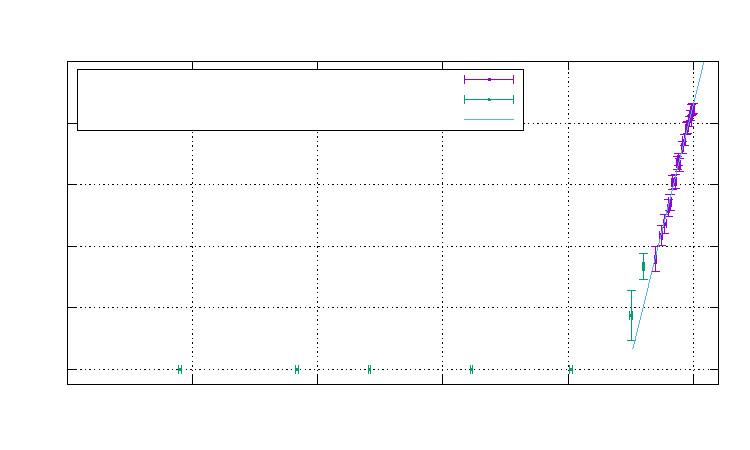
\includegraphics[width={360.00bp},height={216.00bp}]{546nm}}%
    \gplfronttext
  \end{picture}%
\endgroup
}
        \caption{Photostrom abzüglich des Anodenstroms gegen Gegenspannung für $\lambda =\SI{546}{n m}$. Fit nur an Messdaten quadratisch ab $U_0$ und in quadratischer Abhängigkeit.}
\end{figure}
\begin{figure}[h]
        \centering
        \resizebox{.5\textwidth}{!}{% GNUPLOT: LaTeX picture with Postscript
\begingroup
  \makeatletter
  \providecommand\color[2][]{%
    \GenericError{(gnuplot) \space\space\space\@spaces}{%
      Package color not loaded in conjunction with
      terminal option `colourtext'%
    }{See the gnuplot documentation for explanation.%
    }{Either use 'blacktext' in gnuplot or load the package
      color.sty in LaTeX.}%
    \renewcommand\color[2][]{}%
  }%
  \providecommand\includegraphics[2][]{%
    \GenericError{(gnuplot) \space\space\space\@spaces}{%
      Package graphicx or graphics not loaded%
    }{See the gnuplot documentation for explanation.%
    }{The gnuplot epslatex terminal needs graphicx.sty or graphics.sty.}%
    \renewcommand\includegraphics[2][]{}%
  }%
  \providecommand\rotatebox[2]{#2}%
  \@ifundefined{ifGPcolor}{%
    \newif\ifGPcolor
    \GPcolortrue
  }{}%
  \@ifundefined{ifGPblacktext}{%
    \newif\ifGPblacktext
    \GPblacktexttrue
  }{}%
  % define a \g@addto@macro without @ in the name:
  \let\gplgaddtomacro\g@addto@macro
  % define empty templates for all commands taking text:
  \gdef\gplbacktext{}%
  \gdef\gplfronttext{}%
  \makeatother
  \ifGPblacktext
    % no textcolor at all
    \def\colorrgb#1{}%
    \def\colorgray#1{}%
  \else
    % gray or color?
    \ifGPcolor
      \def\colorrgb#1{\color[rgb]{#1}}%
      \def\colorgray#1{\color[gray]{#1}}%
      \expandafter\def\csname LTw\endcsname{\color{white}}%
      \expandafter\def\csname LTb\endcsname{\color{black}}%
      \expandafter\def\csname LTa\endcsname{\color{black}}%
      \expandafter\def\csname LT0\endcsname{\color[rgb]{1,0,0}}%
      \expandafter\def\csname LT1\endcsname{\color[rgb]{0,1,0}}%
      \expandafter\def\csname LT2\endcsname{\color[rgb]{0,0,1}}%
      \expandafter\def\csname LT3\endcsname{\color[rgb]{1,0,1}}%
      \expandafter\def\csname LT4\endcsname{\color[rgb]{0,1,1}}%
      \expandafter\def\csname LT5\endcsname{\color[rgb]{1,1,0}}%
      \expandafter\def\csname LT6\endcsname{\color[rgb]{0,0,0}}%
      \expandafter\def\csname LT7\endcsname{\color[rgb]{1,0.3,0}}%
      \expandafter\def\csname LT8\endcsname{\color[rgb]{0.5,0.5,0.5}}%
    \else
      % gray
      \def\colorrgb#1{\color{black}}%
      \def\colorgray#1{\color[gray]{#1}}%
      \expandafter\def\csname LTw\endcsname{\color{white}}%
      \expandafter\def\csname LTb\endcsname{\color{black}}%
      \expandafter\def\csname LTa\endcsname{\color{black}}%
      \expandafter\def\csname LT0\endcsname{\color{black}}%
      \expandafter\def\csname LT1\endcsname{\color{black}}%
      \expandafter\def\csname LT2\endcsname{\color{black}}%
      \expandafter\def\csname LT3\endcsname{\color{black}}%
      \expandafter\def\csname LT4\endcsname{\color{black}}%
      \expandafter\def\csname LT5\endcsname{\color{black}}%
      \expandafter\def\csname LT6\endcsname{\color{black}}%
      \expandafter\def\csname LT7\endcsname{\color{black}}%
      \expandafter\def\csname LT8\endcsname{\color{black}}%
    \fi
  \fi
    \setlength{\unitlength}{0.0500bp}%
    \ifx\gptboxheight\undefined%
      \newlength{\gptboxheight}%
      \newlength{\gptboxwidth}%
      \newsavebox{\gptboxtext}%
    \fi%
    \setlength{\fboxrule}{0.5pt}%
    \setlength{\fboxsep}{1pt}%
    \definecolor{tbcol}{rgb}{1,1,1}%
\begin{picture}(7200.00,4320.00)%
    \gplgaddtomacro\gplbacktext{%
      \csname LTb\endcsname%%
      \put(536,766){\makebox(0,0)[r]{\strut{}$0$}}%
      \csname LTb\endcsname%%
      \put(536,1357){\makebox(0,0)[r]{\strut{}$2$}}%
      \csname LTb\endcsname%%
      \put(536,1947){\makebox(0,0)[r]{\strut{}$4$}}%
      \csname LTb\endcsname%%
      \put(536,2538){\makebox(0,0)[r]{\strut{}$6$}}%
      \csname LTb\endcsname%%
      \put(536,3128){\makebox(0,0)[r]{\strut{}$8$}}%
      \csname LTb\endcsname%%
      \put(536,3719){\makebox(0,0)[r]{\strut{}$10$}}%
      \csname LTb\endcsname%%
      \put(634,425){\makebox(0,0){\strut{}$-2.5$}}%
      \csname LTb\endcsname%%
      \put(1836,425){\makebox(0,0){\strut{}$-2$}}%
      \csname LTb\endcsname%%
      \put(3038,425){\makebox(0,0){\strut{}$-1.5$}}%
      \csname LTb\endcsname%%
      \put(4241,425){\makebox(0,0){\strut{}$-1$}}%
      \csname LTb\endcsname%%
      \put(5443,425){\makebox(0,0){\strut{}$-0.5$}}%
      \csname LTb\endcsname%%
      \put(6645,425){\makebox(0,0){\strut{}$0$}}%
    }%
    \gplgaddtomacro\gplfronttext{%
      \csname LTb\endcsname%%
      \put(4354,3448){\makebox(0,0)[r]{\strut{}quadratische Datenpunkte}}%
      \csname LTb\endcsname%%
      \put(4354,3255){\makebox(0,0)[r]{\strut{}nicht quadratische Datenpunkte}}%
      \csname LTb\endcsname%%
      \put(4354,3061){\makebox(0,0)[r]{\strut{}$f(U_G)=\SI{20.88 +- 0.77}{}\cdot U_G + \SI{8.108 +- 0.075}{\milli V}$}}%
      \csname LTb\endcsname%%
      \put(170,2169){\rotatebox{-270.00}{\makebox(0,0){\strut{}$\sqrt{I-I_0}$/mV}}}%
      \csname LTb\endcsname%%
      \put(3760,135){\makebox(0,0){\strut{}$U_G$/V}}%
      \csname LTb\endcsname%%
      \put(3760,4009){\makebox(0,0){\strut{}$\lambda=\SI{578}{\nano m}$: $U_0=\SI{-0.388 +- 0.000}{V}$ und $\chi^2/\text{ddof}=\SI{0.850}{}$}}%
    }%
    \gplbacktext
    \put(0,0){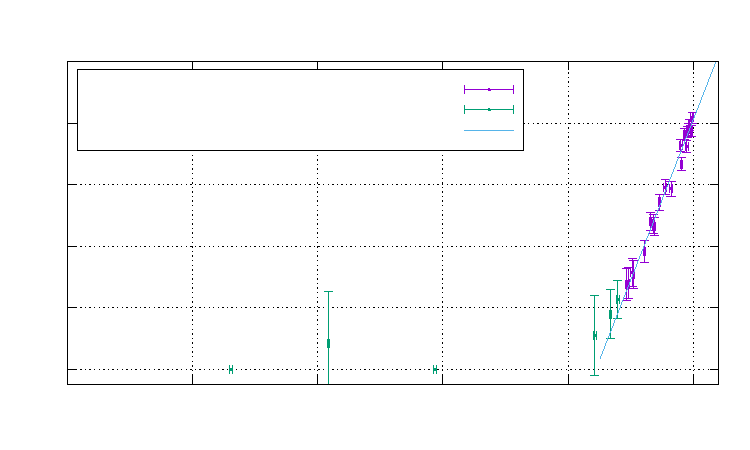
\includegraphics[width={360.00bp},height={216.00bp}]{578nm}}%
    \gplfronttext
  \end{picture}%
\endgroup
}
        \caption{Photostrom abzüglich des Anodenstroms gegen Gegenspannung für $\lambda =\SI{578}{n m}$. Fit nur an Messdaten quadratisch ab $U_0$ und in quadratischer Abhängigkeit.} \label{fig:photo_auswertung_578}
\end{figure}
\begin{figure}[h]
        \centering
        \resizebox{.5\textwidth}{!}{% GNUPLOT: LaTeX picture with Postscript
\begingroup
  \makeatletter
  \providecommand\color[2][]{%
    \GenericError{(gnuplot) \space\space\space\@spaces}{%
      Package color not loaded in conjunction with
      terminal option `colourtext'%
    }{See the gnuplot documentation for explanation.%
    }{Either use 'blacktext' in gnuplot or load the package
      color.sty in LaTeX.}%
    \renewcommand\color[2][]{}%
  }%
  \providecommand\includegraphics[2][]{%
    \GenericError{(gnuplot) \space\space\space\@spaces}{%
      Package graphicx or graphics not loaded%
    }{See the gnuplot documentation for explanation.%
    }{The gnuplot epslatex terminal needs graphicx.sty or graphics.sty.}%
    \renewcommand\includegraphics[2][]{}%
  }%
  \providecommand\rotatebox[2]{#2}%
  \@ifundefined{ifGPcolor}{%
    \newif\ifGPcolor
    \GPcolortrue
  }{}%
  \@ifundefined{ifGPblacktext}{%
    \newif\ifGPblacktext
    \GPblacktexttrue
  }{}%
  % define a \g@addto@macro without @ in the name:
  \let\gplgaddtomacro\g@addto@macro
  % define empty templates for all commands taking text:
  \gdef\gplbacktext{}%
  \gdef\gplfronttext{}%
  \makeatother
  \ifGPblacktext
    % no textcolor at all
    \def\colorrgb#1{}%
    \def\colorgray#1{}%
  \else
    % gray or color?
    \ifGPcolor
      \def\colorrgb#1{\color[rgb]{#1}}%
      \def\colorgray#1{\color[gray]{#1}}%
      \expandafter\def\csname LTw\endcsname{\color{white}}%
      \expandafter\def\csname LTb\endcsname{\color{black}}%
      \expandafter\def\csname LTa\endcsname{\color{black}}%
      \expandafter\def\csname LT0\endcsname{\color[rgb]{1,0,0}}%
      \expandafter\def\csname LT1\endcsname{\color[rgb]{0,1,0}}%
      \expandafter\def\csname LT2\endcsname{\color[rgb]{0,0,1}}%
      \expandafter\def\csname LT3\endcsname{\color[rgb]{1,0,1}}%
      \expandafter\def\csname LT4\endcsname{\color[rgb]{0,1,1}}%
      \expandafter\def\csname LT5\endcsname{\color[rgb]{1,1,0}}%
      \expandafter\def\csname LT6\endcsname{\color[rgb]{0,0,0}}%
      \expandafter\def\csname LT7\endcsname{\color[rgb]{1,0.3,0}}%
      \expandafter\def\csname LT8\endcsname{\color[rgb]{0.5,0.5,0.5}}%
    \else
      % gray
      \def\colorrgb#1{\color{black}}%
      \def\colorgray#1{\color[gray]{#1}}%
      \expandafter\def\csname LTw\endcsname{\color{white}}%
      \expandafter\def\csname LTb\endcsname{\color{black}}%
      \expandafter\def\csname LTa\endcsname{\color{black}}%
      \expandafter\def\csname LT0\endcsname{\color{black}}%
      \expandafter\def\csname LT1\endcsname{\color{black}}%
      \expandafter\def\csname LT2\endcsname{\color{black}}%
      \expandafter\def\csname LT3\endcsname{\color{black}}%
      \expandafter\def\csname LT4\endcsname{\color{black}}%
      \expandafter\def\csname LT5\endcsname{\color{black}}%
      \expandafter\def\csname LT6\endcsname{\color{black}}%
      \expandafter\def\csname LT7\endcsname{\color{black}}%
      \expandafter\def\csname LT8\endcsname{\color{black}}%
    \fi
  \fi
    \setlength{\unitlength}{0.0500bp}%
    \ifx\gptboxheight\undefined%
      \newlength{\gptboxheight}%
      \newlength{\gptboxwidth}%
      \newsavebox{\gptboxtext}%
    \fi%
    \setlength{\fboxrule}{0.5pt}%
    \setlength{\fboxsep}{1pt}%
    \definecolor{tbcol}{rgb}{1,1,1}%
\begin{picture}(7200.00,4320.00)%
    \gplgaddtomacro\gplbacktext{%
      \csname LTb\endcsname%%
      \put(634,619){\makebox(0,0)[r]{\strut{}$0$}}%
      \csname LTb\endcsname%%
      \put(634,1239){\makebox(0,0)[r]{\strut{}$20$}}%
      \csname LTb\endcsname%%
      \put(634,1859){\makebox(0,0)[r]{\strut{}$40$}}%
      \csname LTb\endcsname%%
      \put(634,2479){\makebox(0,0)[r]{\strut{}$60$}}%
      \csname LTb\endcsname%%
      \put(634,3099){\makebox(0,0)[r]{\strut{}$80$}}%
      \csname LTb\endcsname%%
      \put(634,3719){\makebox(0,0)[r]{\strut{}$100$}}%
      \csname LTb\endcsname%%
      \put(731,425){\makebox(0,0){\strut{}$-0.1$}}%
      \csname LTb\endcsname%%
      \put(2270,425){\makebox(0,0){\strut{}$-0.05$}}%
      \csname LTb\endcsname%%
      \put(3809,425){\makebox(0,0){\strut{}$0$}}%
      \csname LTb\endcsname%%
      \put(5347,425){\makebox(0,0){\strut{}$0.05$}}%
      \csname LTb\endcsname%%
      \put(6886,425){\makebox(0,0){\strut{}$0.1$}}%
    }%
    \gplgaddtomacro\gplfronttext{%
      \csname LTb\endcsname%%
      \put(170,2169){\rotatebox{-270}{\makebox(0,0){\strut{}Intensität $I/\%$}}}%
      \csname LTb\endcsname%%
      \put(3809,135){\makebox(0,0){\strut{}relativer Winkel $\Delta\omega_G/\SI{}{\degree}$}}%
      \csname LTb\endcsname%%
      \put(2592,3448){\makebox(0,0)[r]{\strut{}Rote Aufspaltung}}%
      \csname LTb\endcsname%%
      \put(2592,3255){\makebox(0,0)[r]{\strut{}$f(x)$}}%
      \csname LTb\endcsname%%
      \put(3809,4009){\makebox(0,0){\strut{}Isotopieaufspaltung von Wasserstoff und Deuterium bei $\lambda=\SI{656}{\nano m}$}}%
    }%
    \gplbacktext
    \put(0,0){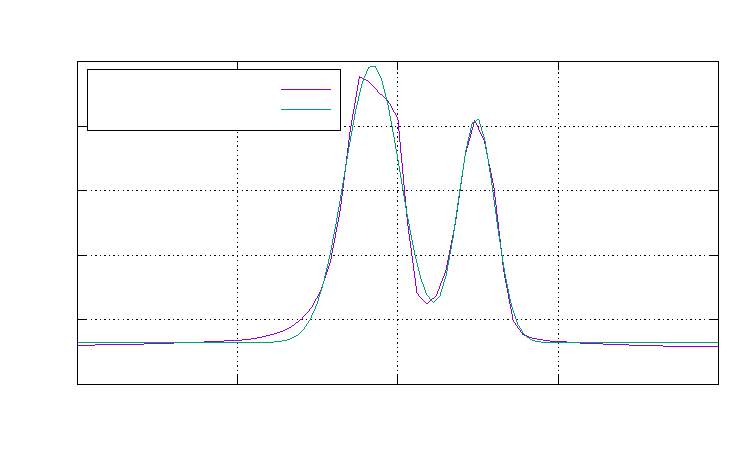
\includegraphics[width={360.00bp},height={216.00bp}]{ccdrot}}%
    \gplfronttext
  \end{picture}%
\endgroup
}
        \caption{Rote Isotopieaufspaltung der \textsc{Balmer}--Lampe gemessen mit der CCD.} \label{fig:ccdrot}
\end{figure}
\begin{figure}[h]
        \centering
        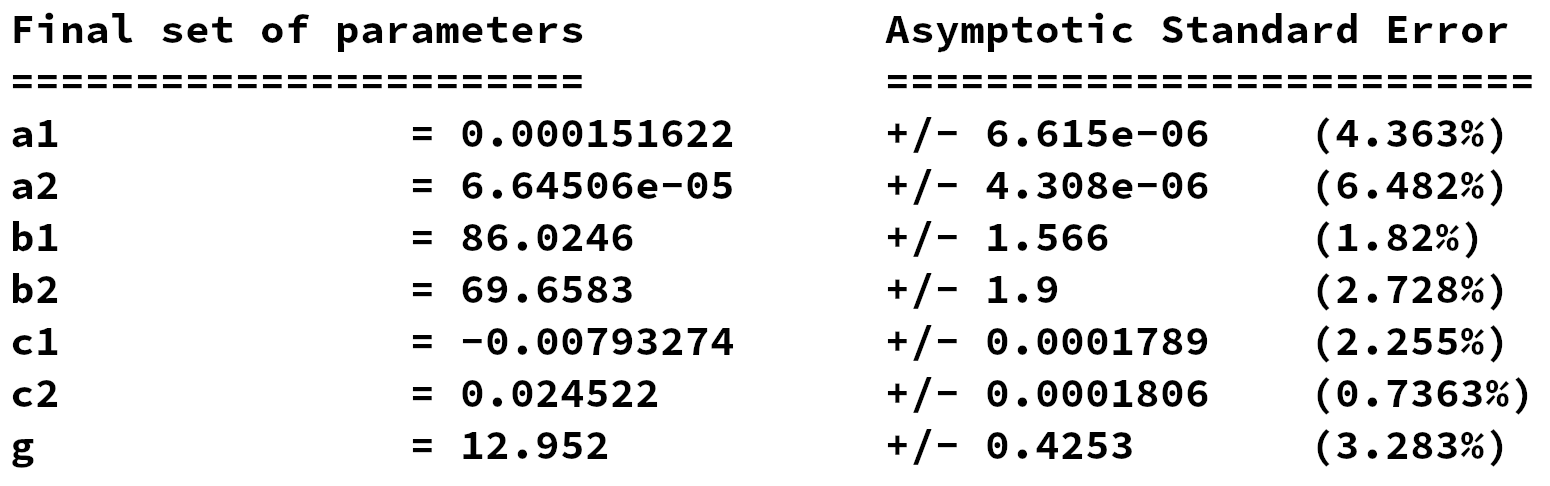
\includegraphics[width=.5\textwidth]{ccdrot_params.png}
        \caption{Fitparameter der roten Isotopieaufspaltung.}
\end{figure}
\begin{figure}[h]
        \centering
        \resizebox{.5\textwidth}{!}{% GNUPLOT: LaTeX picture with Postscript
\documentclass{minimal}
% Set font size
\makeatletter
\def\@ptsize{1}
\InputIfFileExists{size11.clo}{}{%
   \GenericError{(gnuplot) \space\space\space\@spaces}{%
      Gnuplot Error: File `size11.clo' not found! Could not set font size%
   }{See the gnuplot documentation for explanation.%
   }{For using a font size a file `size<fontsize>.clo' has to exist.
        Falling back ^^Jto default fontsize 10pt.}%
  \def\@ptsize{0}
  \input{size10.clo}%
}%
\makeatother
% Load packages
\usepackage{calc}
\usepackage{graphicx}
\usepackage{color}
\usepackage{transparent}
\makeatletter
% Select an appropriate default driver (from TeXLive graphics.cfg)
\begingroup
  \chardef\x=0 %
  % check pdfTeX
  \@ifundefined{pdfoutput}{}{%
    \ifcase\pdfoutput
    \else
      \chardef\x=1 %
    \fi
  }%
  % check VTeX
  \@ifundefined{OpMode}{}{%
    \chardef\x=2 %
  }%
\expandafter\endgroup
\ifcase\x
  % default case
  \PassOptionsToPackage{dvips}{geometry}
\or
  % pdfTeX is running in pdf mode
  \PassOptionsToPackage{pdftex}{geometry}
\else
  % VTeX is running
  \PassOptionsToPackage{vtex}{geometry}
\fi
\makeatother
% Set papersize
\usepackage[papersize={360.00bp,216.00bp},text={360.00bp,216.00bp}]{geometry}
% No page numbers and no paragraph indentation
\pagestyle{empty}
\setlength{\parindent}{0bp}%
% Load configuration file
\InputIfFileExists{gnuplot.cfg}{%
  \typeout{Using configuration file gnuplot.cfg}%
}{%
 \typeout{No configuration file gnuplot.cfg found.}%
}%
\usepackage{siunitx}
\begin{document}
\begingroup
  \makeatletter
  \providecommand\color[2][]{%
    \GenericError{(gnuplot) \space\space\space\@spaces}{%
      Package color not loaded in conjunction with
      terminal option `colourtext'%
    }{See the gnuplot documentation for explanation.%
    }{Either use 'blacktext' in gnuplot or load the package
      color.sty in LaTeX.}%
    \renewcommand\color[2][]{}%
  }%
  \providecommand\includegraphics[2][]{%
    \GenericError{(gnuplot) \space\space\space\@spaces}{%
      Package graphicx or graphics not loaded%
    }{See the gnuplot documentation for explanation.%
    }{The gnuplot epslatex terminal needs graphicx.sty or graphics.sty.}%
    \renewcommand\includegraphics[2][]{}%
  }%
  \providecommand\rotatebox[2]{#2}%
  \@ifundefined{ifGPcolor}{%
    \newif\ifGPcolor
    \GPcolortrue
  }{}%
  \@ifundefined{ifGPblacktext}{%
    \newif\ifGPblacktext
    \GPblacktexttrue
  }{}%
  % define a \g@addto@macro without @ in the name:
  \let\gplgaddtomacro\g@addto@macro
  % define empty templates for all commands taking text:
  \gdef\gplbacktext{}%
  \gdef\gplfronttext{}%
  \makeatother
  \ifGPblacktext
    % no textcolor at all
    \def\colorrgb#1{}%
    \def\colorgray#1{}%
  \else
    % gray or color?
    \ifGPcolor
      \def\colorrgb#1{\color[rgb]{#1}}%
      \def\colorgray#1{\color[gray]{#1}}%
      \expandafter\def\csname LTw\endcsname{\color{white}}%
      \expandafter\def\csname LTb\endcsname{\color{black}}%
      \expandafter\def\csname LTa\endcsname{\color{black}}%
      \expandafter\def\csname LT0\endcsname{\color[rgb]{1,0,0}}%
      \expandafter\def\csname LT1\endcsname{\color[rgb]{0,1,0}}%
      \expandafter\def\csname LT2\endcsname{\color[rgb]{0,0,1}}%
      \expandafter\def\csname LT3\endcsname{\color[rgb]{1,0,1}}%
      \expandafter\def\csname LT4\endcsname{\color[rgb]{0,1,1}}%
      \expandafter\def\csname LT5\endcsname{\color[rgb]{1,1,0}}%
      \expandafter\def\csname LT6\endcsname{\color[rgb]{0,0,0}}%
      \expandafter\def\csname LT7\endcsname{\color[rgb]{1,0.3,0}}%
      \expandafter\def\csname LT8\endcsname{\color[rgb]{0.5,0.5,0.5}}%
    \else
      % gray
      \def\colorrgb#1{\color{black}}%
      \def\colorgray#1{\color[gray]{#1}}%
      \expandafter\def\csname LTw\endcsname{\color{white}}%
      \expandafter\def\csname LTb\endcsname{\color{black}}%
      \expandafter\def\csname LTa\endcsname{\color{black}}%
      \expandafter\def\csname LT0\endcsname{\color{black}}%
      \expandafter\def\csname LT1\endcsname{\color{black}}%
      \expandafter\def\csname LT2\endcsname{\color{black}}%
      \expandafter\def\csname LT3\endcsname{\color{black}}%
      \expandafter\def\csname LT4\endcsname{\color{black}}%
      \expandafter\def\csname LT5\endcsname{\color{black}}%
      \expandafter\def\csname LT6\endcsname{\color{black}}%
      \expandafter\def\csname LT7\endcsname{\color{black}}%
      \expandafter\def\csname LT8\endcsname{\color{black}}%
    \fi
  \fi
    \setlength{\unitlength}{0.0500bp}%
    \ifx\gptboxheight\undefined%
      \newlength{\gptboxheight}%
      \newlength{\gptboxwidth}%
      \newsavebox{\gptboxtext}%
    \fi%
    \setlength{\fboxrule}{0.5pt}%
    \setlength{\fboxsep}{1pt}%
    \definecolor{tbcol}{rgb}{1,1,1}%
\begin{picture}(7200.00,4320.00)%
    \gplgaddtomacro\gplbacktext{%
      \csname LTb\endcsname%%
      \put(634,619){\makebox(0,0)[r]{\strut{}$0$}}%
      \csname LTb\endcsname%%
      \put(634,1239){\makebox(0,0)[r]{\strut{}$20$}}%
      \csname LTb\endcsname%%
      \put(634,1859){\makebox(0,0)[r]{\strut{}$40$}}%
      \csname LTb\endcsname%%
      \put(634,2479){\makebox(0,0)[r]{\strut{}$60$}}%
      \csname LTb\endcsname%%
      \put(634,3099){\makebox(0,0)[r]{\strut{}$80$}}%
      \csname LTb\endcsname%%
      \put(634,3719){\makebox(0,0)[r]{\strut{}$100$}}%
      \csname LTb\endcsname%%
      \put(731,425){\makebox(0,0){\strut{}$-0.1$}}%
      \csname LTb\endcsname%%
      \put(2270,425){\makebox(0,0){\strut{}$-0.05$}}%
      \csname LTb\endcsname%%
      \put(3809,425){\makebox(0,0){\strut{}$0$}}%
      \csname LTb\endcsname%%
      \put(5347,425){\makebox(0,0){\strut{}$0.05$}}%
      \csname LTb\endcsname%%
      \put(6886,425){\makebox(0,0){\strut{}$0.1$}}%
    }%
    \gplgaddtomacro\gplfronttext{%
      \csname LTb\endcsname%%
      \put(4749,1083){\makebox(0,0)[r]{\strut{}Turkisfarbene Aufspaltung}}%
      \csname LTb\endcsname%%
      \put(4749,890){\makebox(0,0)[r]{\strut{}$f(x)$}}%
      \csname LTb\endcsname%%
      \put(170,2169){\rotatebox{-270.00}{\makebox(0,0){\strut{}Intensität $I/\%$}}}%
      \csname LTb\endcsname%%
      \put(3809,135){\makebox(0,0){\strut{}relativer Winkel $\Delta\omega_G/\SI{}{\degree}$}}%
      \csname LTb\endcsname%%
      \put(3809,4009){\makebox(0,0){\strut{}Isotopieaufspaltung von Wasserstoff und Deuterium bei $\lambda=\SI{486}{\nano m}$}}%
    }%
    \gplbacktext
    \put(0,0){\includegraphics[width={360.00bp},height={216.00bp}]{ccdtuerkis-inc}}%
    \gplfronttext
  \end{picture}%
\endgroup
\end{document}
}
        \caption{Türkisfarbene Isotopieaufspaltung der \textsc{Balmer}--Lampe gemessen mit der CCD.} \label{fig:ccdtürkis}
\end{figure}
\begin{figure}[h]
        \centering
        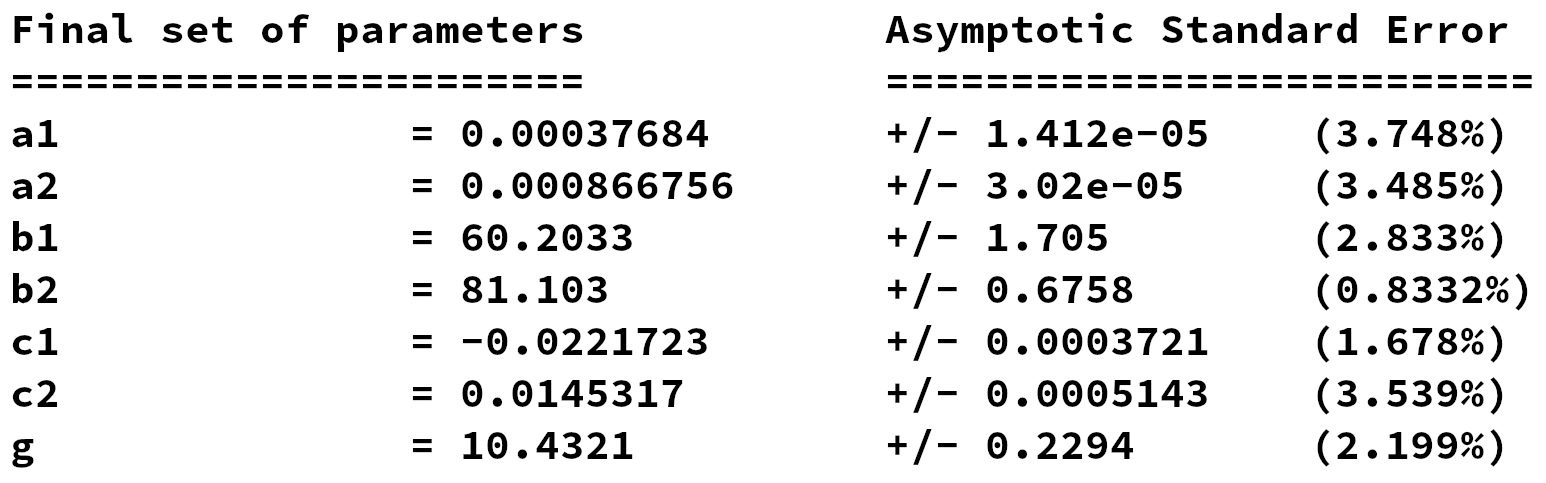
\includegraphics[width=.5\textwidth]{ccdtuerkis_params.png}
        \caption{Fitparameter der türkisfarbenen Isotopieaufspaltung.}
\end{figure}
\begin{figure}[h]
        \centering
        \resizebox{.5\textwidth}{!}{% GNUPLOT: LaTeX picture with Postscript
\begingroup
  \makeatletter
  \providecommand\color[2][]{%
    \GenericError{(gnuplot) \space\space\space\@spaces}{%
      Package color not loaded in conjunction with
      terminal option `colourtext'%
    }{See the gnuplot documentation for explanation.%
    }{Either use 'blacktext' in gnuplot or load the package
      color.sty in LaTeX.}%
    \renewcommand\color[2][]{}%
  }%
  \providecommand\includegraphics[2][]{%
    \GenericError{(gnuplot) \space\space\space\@spaces}{%
      Package graphicx or graphics not loaded%
    }{See the gnuplot documentation for explanation.%
    }{The gnuplot epslatex terminal needs graphicx.sty or graphics.sty.}%
    \renewcommand\includegraphics[2][]{}%
  }%
  \providecommand\rotatebox[2]{#2}%
  \@ifundefined{ifGPcolor}{%
    \newif\ifGPcolor
    \GPcolortrue
  }{}%
  \@ifundefined{ifGPblacktext}{%
    \newif\ifGPblacktext
    \GPblacktexttrue
  }{}%
  % define a \g@addto@macro without @ in the name:
  \let\gplgaddtomacro\g@addto@macro
  % define empty templates for all commands taking text:
  \gdef\gplbacktext{}%
  \gdef\gplfronttext{}%
  \makeatother
  \ifGPblacktext
    % no textcolor at all
    \def\colorrgb#1{}%
    \def\colorgray#1{}%
  \else
    % gray or color?
    \ifGPcolor
      \def\colorrgb#1{\color[rgb]{#1}}%
      \def\colorgray#1{\color[gray]{#1}}%
      \expandafter\def\csname LTw\endcsname{\color{white}}%
      \expandafter\def\csname LTb\endcsname{\color{black}}%
      \expandafter\def\csname LTa\endcsname{\color{black}}%
      \expandafter\def\csname LT0\endcsname{\color[rgb]{1,0,0}}%
      \expandafter\def\csname LT1\endcsname{\color[rgb]{0,1,0}}%
      \expandafter\def\csname LT2\endcsname{\color[rgb]{0,0,1}}%
      \expandafter\def\csname LT3\endcsname{\color[rgb]{1,0,1}}%
      \expandafter\def\csname LT4\endcsname{\color[rgb]{0,1,1}}%
      \expandafter\def\csname LT5\endcsname{\color[rgb]{1,1,0}}%
      \expandafter\def\csname LT6\endcsname{\color[rgb]{0,0,0}}%
      \expandafter\def\csname LT7\endcsname{\color[rgb]{1,0.3,0}}%
      \expandafter\def\csname LT8\endcsname{\color[rgb]{0.5,0.5,0.5}}%
    \else
      % gray
      \def\colorrgb#1{\color{black}}%
      \def\colorgray#1{\color[gray]{#1}}%
      \expandafter\def\csname LTw\endcsname{\color{white}}%
      \expandafter\def\csname LTb\endcsname{\color{black}}%
      \expandafter\def\csname LTa\endcsname{\color{black}}%
      \expandafter\def\csname LT0\endcsname{\color{black}}%
      \expandafter\def\csname LT1\endcsname{\color{black}}%
      \expandafter\def\csname LT2\endcsname{\color{black}}%
      \expandafter\def\csname LT3\endcsname{\color{black}}%
      \expandafter\def\csname LT4\endcsname{\color{black}}%
      \expandafter\def\csname LT5\endcsname{\color{black}}%
      \expandafter\def\csname LT6\endcsname{\color{black}}%
      \expandafter\def\csname LT7\endcsname{\color{black}}%
      \expandafter\def\csname LT8\endcsname{\color{black}}%
    \fi
  \fi
    \setlength{\unitlength}{0.0500bp}%
    \ifx\gptboxheight\undefined%
      \newlength{\gptboxheight}%
      \newlength{\gptboxwidth}%
      \newsavebox{\gptboxtext}%
    \fi%
    \setlength{\fboxrule}{0.5pt}%
    \setlength{\fboxsep}{1pt}%
    \definecolor{tbcol}{rgb}{1,1,1}%
\begin{picture}(7200.00,4320.00)%
    \gplgaddtomacro\gplbacktext{%
      \csname LTb\endcsname%%
      \put(634,619){\makebox(0,0)[r]{\strut{}$0$}}%
      \csname LTb\endcsname%%
      \put(634,1239){\makebox(0,0)[r]{\strut{}$20$}}%
      \csname LTb\endcsname%%
      \put(634,1859){\makebox(0,0)[r]{\strut{}$40$}}%
      \csname LTb\endcsname%%
      \put(634,2479){\makebox(0,0)[r]{\strut{}$60$}}%
      \csname LTb\endcsname%%
      \put(634,3099){\makebox(0,0)[r]{\strut{}$80$}}%
      \csname LTb\endcsname%%
      \put(634,3719){\makebox(0,0)[r]{\strut{}$100$}}%
      \csname LTb\endcsname%%
      \put(731,425){\makebox(0,0){\strut{}$-0.1$}}%
      \csname LTb\endcsname%%
      \put(2270,425){\makebox(0,0){\strut{}$-0.05$}}%
      \csname LTb\endcsname%%
      \put(3809,425){\makebox(0,0){\strut{}$0$}}%
      \csname LTb\endcsname%%
      \put(5347,425){\makebox(0,0){\strut{}$0.05$}}%
      \csname LTb\endcsname%%
      \put(6886,425){\makebox(0,0){\strut{}$0.1$}}%
    }%
    \gplgaddtomacro\gplfronttext{%
      \csname LTb\endcsname%%
      \put(170,2169){\rotatebox{-270}{\makebox(0,0){\strut{}Intensität $I/\%$}}}%
      \csname LTb\endcsname%%
      \put(3809,135){\makebox(0,0){\strut{}relativer Winkel $\Delta\omega_G/\SI{}{\degree}$}}%
      \csname LTb\endcsname%%
      \put(4452,3448){\makebox(0,0)[r]{\strut{}Violetfarbene (schwache) Aufspaltung}}%
      \csname LTb\endcsname%%
      \put(4452,3255){\makebox(0,0)[r]{\strut{}$f(x)$}}%
      \csname LTb\endcsname%%
      \put(3809,4009){\makebox(0,0){\strut{}Isotopieaufspaltung von Wasserstoff und Deuterium bei $\lambda=\SI{434}{\nano m}$}}%
    }%
    \gplbacktext
    \put(0,0){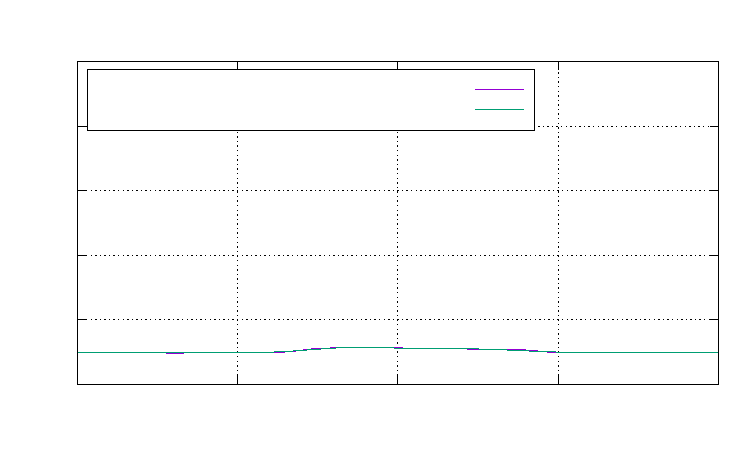
\includegraphics[width={360.00bp},height={216.00bp}]{ccdvioletschwach}}%
    \gplfronttext
  \end{picture}%
\endgroup
}
        \caption{Schwache violetfarbene Isotopieaufspaltung der \textsc{Balmer}--Lampe gemessen mit der CCD.} \label{fig:ccdvioletschwach}
\end{figure}
\begin{figure}[h]
        \centering
        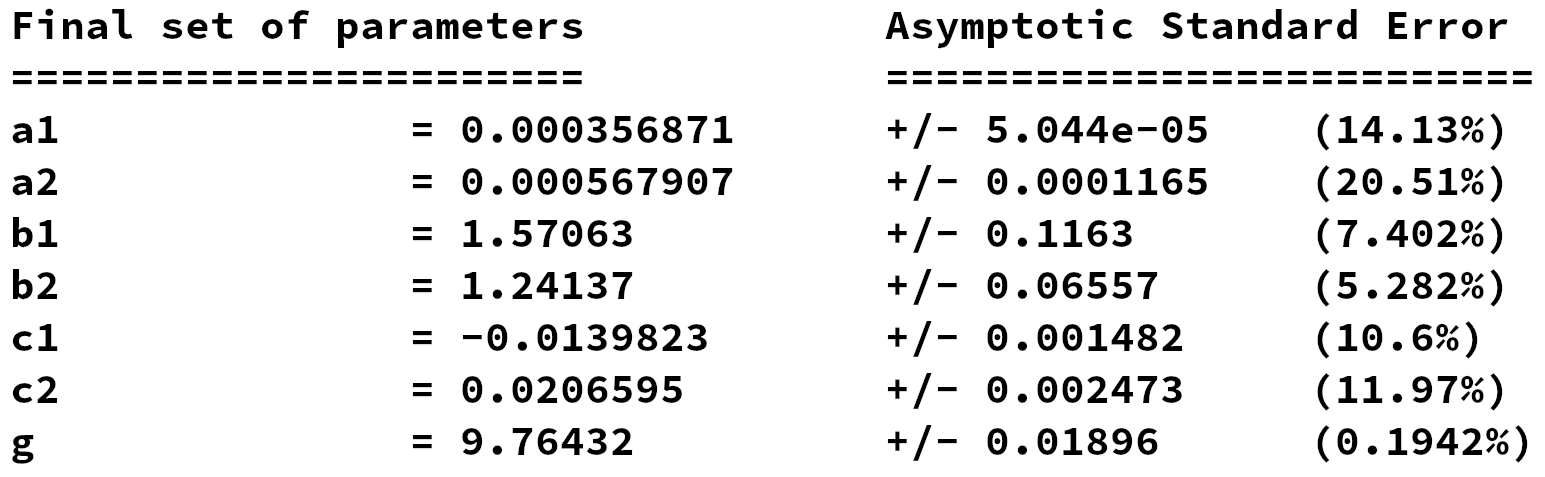
\includegraphics[width=.5\textwidth]{ccdvioletschwach_params.png}
        \caption{Fitparameter der schwachen violetfarbenen Isotopieaufspaltung.}
\end{figure}
\begin{figure}[h]
        \centering
        \resizebox{.5\textwidth}{!}{% GNUPLOT: LaTeX picture with Postscript
\begingroup
  \makeatletter
  \providecommand\color[2][]{%
    \GenericError{(gnuplot) \space\space\space\@spaces}{%
      Package color not loaded in conjunction with
      terminal option `colourtext'%
    }{See the gnuplot documentation for explanation.%
    }{Either use 'blacktext' in gnuplot or load the package
      color.sty in LaTeX.}%
    \renewcommand\color[2][]{}%
  }%
  \providecommand\includegraphics[2][]{%
    \GenericError{(gnuplot) \space\space\space\@spaces}{%
      Package graphicx or graphics not loaded%
    }{See the gnuplot documentation for explanation.%
    }{The gnuplot epslatex terminal needs graphicx.sty or graphics.sty.}%
    \renewcommand\includegraphics[2][]{}%
  }%
  \providecommand\rotatebox[2]{#2}%
  \@ifundefined{ifGPcolor}{%
    \newif\ifGPcolor
    \GPcolortrue
  }{}%
  \@ifundefined{ifGPblacktext}{%
    \newif\ifGPblacktext
    \GPblacktexttrue
  }{}%
  % define a \g@addto@macro without @ in the name:
  \let\gplgaddtomacro\g@addto@macro
  % define empty templates for all commands taking text:
  \gdef\gplbacktext{}%
  \gdef\gplfronttext{}%
  \makeatother
  \ifGPblacktext
    % no textcolor at all
    \def\colorrgb#1{}%
    \def\colorgray#1{}%
  \else
    % gray or color?
    \ifGPcolor
      \def\colorrgb#1{\color[rgb]{#1}}%
      \def\colorgray#1{\color[gray]{#1}}%
      \expandafter\def\csname LTw\endcsname{\color{white}}%
      \expandafter\def\csname LTb\endcsname{\color{black}}%
      \expandafter\def\csname LTa\endcsname{\color{black}}%
      \expandafter\def\csname LT0\endcsname{\color[rgb]{1,0,0}}%
      \expandafter\def\csname LT1\endcsname{\color[rgb]{0,1,0}}%
      \expandafter\def\csname LT2\endcsname{\color[rgb]{0,0,1}}%
      \expandafter\def\csname LT3\endcsname{\color[rgb]{1,0,1}}%
      \expandafter\def\csname LT4\endcsname{\color[rgb]{0,1,1}}%
      \expandafter\def\csname LT5\endcsname{\color[rgb]{1,1,0}}%
      \expandafter\def\csname LT6\endcsname{\color[rgb]{0,0,0}}%
      \expandafter\def\csname LT7\endcsname{\color[rgb]{1,0.3,0}}%
      \expandafter\def\csname LT8\endcsname{\color[rgb]{0.5,0.5,0.5}}%
    \else
      % gray
      \def\colorrgb#1{\color{black}}%
      \def\colorgray#1{\color[gray]{#1}}%
      \expandafter\def\csname LTw\endcsname{\color{white}}%
      \expandafter\def\csname LTb\endcsname{\color{black}}%
      \expandafter\def\csname LTa\endcsname{\color{black}}%
      \expandafter\def\csname LT0\endcsname{\color{black}}%
      \expandafter\def\csname LT1\endcsname{\color{black}}%
      \expandafter\def\csname LT2\endcsname{\color{black}}%
      \expandafter\def\csname LT3\endcsname{\color{black}}%
      \expandafter\def\csname LT4\endcsname{\color{black}}%
      \expandafter\def\csname LT5\endcsname{\color{black}}%
      \expandafter\def\csname LT6\endcsname{\color{black}}%
      \expandafter\def\csname LT7\endcsname{\color{black}}%
      \expandafter\def\csname LT8\endcsname{\color{black}}%
    \fi
  \fi
    \setlength{\unitlength}{0.0500bp}%
    \ifx\gptboxheight\undefined%
      \newlength{\gptboxheight}%
      \newlength{\gptboxwidth}%
      \newsavebox{\gptboxtext}%
    \fi%
    \setlength{\fboxrule}{0.5pt}%
    \setlength{\fboxsep}{1pt}%
    \definecolor{tbcol}{rgb}{1,1,1}%
\begin{picture}(7200.00,4320.00)%
    \gplgaddtomacro\gplbacktext{%
      \csname LTb\endcsname%%
      \put(634,619){\makebox(0,0)[r]{\strut{}$0$}}%
      \csname LTb\endcsname%%
      \put(634,1239){\makebox(0,0)[r]{\strut{}$20$}}%
      \csname LTb\endcsname%%
      \put(634,1859){\makebox(0,0)[r]{\strut{}$40$}}%
      \csname LTb\endcsname%%
      \put(634,2479){\makebox(0,0)[r]{\strut{}$60$}}%
      \csname LTb\endcsname%%
      \put(634,3099){\makebox(0,0)[r]{\strut{}$80$}}%
      \csname LTb\endcsname%%
      \put(634,3719){\makebox(0,0)[r]{\strut{}$100$}}%
      \csname LTb\endcsname%%
      \put(731,425){\makebox(0,0){\strut{}$-0.1$}}%
      \csname LTb\endcsname%%
      \put(2270,425){\makebox(0,0){\strut{}$-0.05$}}%
      \csname LTb\endcsname%%
      \put(3809,425){\makebox(0,0){\strut{}$0$}}%
      \csname LTb\endcsname%%
      \put(5347,425){\makebox(0,0){\strut{}$0.05$}}%
      \csname LTb\endcsname%%
      \put(6886,425){\makebox(0,0){\strut{}$0.1$}}%
    }%
    \gplgaddtomacro\gplfronttext{%
      \csname LTb\endcsname%%
      \put(170,2169){\rotatebox{-270}{\makebox(0,0){\strut{}Intensität $I/\%$}}}%
      \csname LTb\endcsname%%
      \put(3809,135){\makebox(0,0){\strut{}relativer Winkel $\Delta\omega_G/\SI{}{\degree}$}}%
      \csname LTb\endcsname%%
      \put(2592,3448){\makebox(0,0)[r]{\strut{}Rote Aufspaltung}}%
      \csname LTb\endcsname%%
      \put(2592,3255){\makebox(0,0)[r]{\strut{}$f(x)$}}%
      \csname LTb\endcsname%%
      \put(3809,4009){\makebox(0,0){\strut{}Isotopieaufspaltung von Wasserstoff und Deuterium bei $\lambda=\SI{656}{\nano m}$}}%
    }%
    \gplbacktext
    \put(0,0){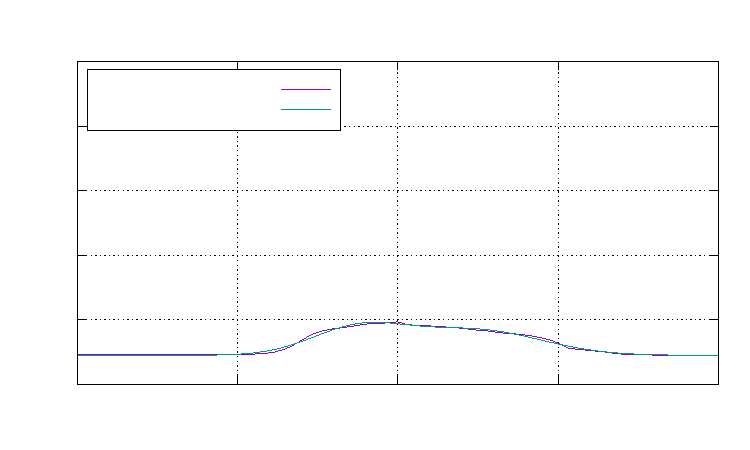
\includegraphics[width={360.00bp},height={216.00bp}]{ccdvioletstark}}%
    \gplfronttext
  \end{picture}%
\endgroup
}
        \caption{Starke violetfarbene Isotopieaufspaltung der \textsc{Balmer}--Lampe gemessen mit der CCD.} \label{fig:ccdvioletstark}
\end{figure}
\begin{figure}[h]
        \centering
        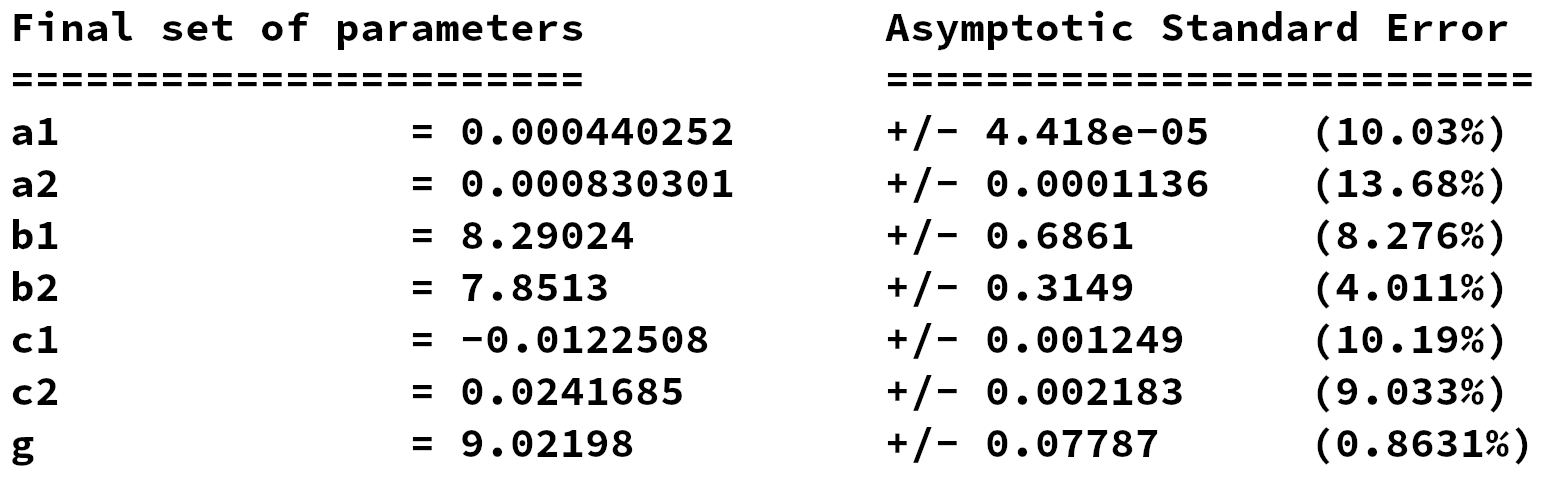
\includegraphics[width=.5\textwidth]{ccdvioletstark_params.png}
        \caption{Fitparameter der starken violetfarbenen Isotopieaufspaltung.}
\end{figure}

\clearpage
\bibliography{refs}
%}}}

\end{document}
